\documentclass[12pt]{article}

\usepackage[a4paper, margin=1in]{geometry}
\usepackage[english]{babel}
\usepackage[utf8]{inputenc}
%\usepackage{fancyhdr}

%\pagestyle{fancy}
%\fancyhf{}
%\fancyhead[L]{\rightmark}
%\fancyhead[R]{\thepage}
%\renewcommand{\headrulewidth}{0pt}
%\renewcommand{\sectionmark}[1]{\markboth{}{{\thesection~#1}}
%\renewcommand{\subsectionmark}[1]{}% Remove \subsection from header

% Copyright 2017 Sergei Tikhomirov, MIT License
% https://github.com/s-tikhomirov/solidity-latex-highlighting/

\usepackage{listings, xcolor}

\definecolor{verylightgray}{rgb}{.97,.97,.97}

\lstdefinelanguage{Solidity}{
	keywords=[1]{anonymous, assembly, assert, balance, break, call, callcode, case, catch, class, constant, continue, constructor, contract, debugger, default, delegatecall, delete, do, else, emit, event, experimental, export, external, false, finally, for, function, gas, if, implements, import, in, indexed, instanceof, interface, internal, is, length, library, log0, log1, log2, log3, log4, memory, modifier, new, payable, pragma, private, protected, public, pure, push, require, return, returns, revert, selfdestruct, send, solidity, storage, struct, suicide, super, switch, then, this, throw, transfer, true, try, typeof, using, value, view, while, with, addmod, ecrecover, keccak256, mulmod, ripemd160, sha256, sha3}, % generic keywords including crypto operations
	keywordstyle=[1]\color{blue}\bfseries,
	keywords=[2]{address, bool, byte, bytes, bytes1, bytes2, bytes3, bytes4, bytes5, bytes6, bytes7, bytes8, bytes9, bytes10, bytes11, bytes12, bytes13, bytes14, bytes15, bytes16, bytes17, bytes18, bytes19, bytes20, bytes21, bytes22, bytes23, bytes24, bytes25, bytes26, bytes27, bytes28, bytes29, bytes30, bytes31, bytes32, enum, int, int8, int16, int24, int32, int40, int48, int56, int64, int72, int80, int88, int96, int104, int112, int120, int128, int136, int144, int152, int160, int168, int176, int184, int192, int200, int208, int216, int224, int232, int240, int248, int256, mapping, string, uint, uint8, uint16, uint24, uint32, uint40, uint48, uint56, uint64, uint72, uint80, uint88, uint96, uint104, uint112, uint120, uint128, uint136, uint144, uint152, uint160, uint168, uint176, uint184, uint192, uint200, uint208, uint216, uint224, uint232, uint240, uint248, uint256, var, void, ether, finney, szabo, wei, days, hours, minutes, seconds, weeks, years},	% types; money and time units
	keywordstyle=[2]\color{teal}\bfseries,
	keywords=[3]{block, blockhash, coinbase, difficulty, gaslimit, number, timestamp, msg, data, gas, sender, sig, value, now, tx, gasprice, origin},	% environment variables
	keywordstyle=[3]\color{violet}\bfseries,
	identifierstyle=\color{black},
	sensitive=false,
	comment=[l]{//},
	morecomment=[s]{/*}{*/},
	commentstyle=\color{gray}\ttfamily,
	stringstyle=\color{red}\ttfamily,
	morestring=[b]',
	morestring=[b]"
}

\lstset{
	language=Solidity,
	backgroundcolor=\color{verylightgray},
	extendedchars=true,
	basicstyle=\footnotesize\ttfamily,
	showstringspaces=false,
	showspaces=false,
	numbers=left,
	numberstyle=\footnotesize,
	numbersep=9pt,
	tabsize=2,
	breaklines=true,
	showtabs=false,
	captionpos=b
}

\usepackage{listings, xcolor}

\definecolor{brilliantrose}{rgb}{1.0, 0.33, 0.64}
\definecolor{electriclime}{rgb}{0.8, 1.0, 0.0}
\definecolor{emerald}{rgb}{0.31, 0.78, 0.47}
\definecolor{amethyst}{rgb}{0.6, 0.4, 0.8}

\lstdefinelanguage{CSharp}
{
 morecomment = [l]{...},
 morecomment = [l]{//}, 
 morecomment = [l]{///},
 morecomment = [s]{/*}{*/},
 morestring=[b]", 
 commentstyle=\color{emerald}\ttfamily,
 sensitive = true,
 morekeywords = {abstract,  event,  new,  struct,
   as,  explicit,  null,  switch,
   base,  extern,  object,  this,
   bool,  false,  operator,  throw,
   break,  finally,  out,  true,
   byte,  fixed,  override,  try,
   case,  float,  params,  typeof,
   catch,  for,  private,  uint,
   char,  foreach,  protected,  ulong,
   checked,  goto,  public,  unchecked,
   class,  if,  readonly,  unsafe,
   const,  implicit,  ref,  ushort,
   continue,  in,  return,  using,
   decimal,  int,  sbyte,  virtual,
   default,  interface,  sealed,  volatile,
   delegate,  internal,  short,  void,
   do,  is,  sizeof,  while,
   double,  lock,  stackalloc, var, await,  
   else,  long,  static,   
   enum,  namespace,  string}
}



\usepackage[colorlinks=true, allcolors=blue]{hyperref}

\title{CRPL: Interim Report}
\author{Harrison Beau Barker}

\usepackage{graphicx,float}
\graphicspath{ {images/} }

\usepackage{xcolor}

\usepackage{tabularx}
\newcolumntype{b}{X}
\newcolumntype{s}{>{\hsize=.5\hsize}X}

\newcommand{\keyword}[1]{\textbf{\textit{#1}}}
\newcommand{\q}[2]{\begin{quote} #1 \cite{#2} \end{quote}}
\newcommand{\nft}[0]{\href{https://eips.ethereum.org/EIPS/eip-721}{EIP-721} }
\newcommand{\br}[0]{\\~\\}

\setlength{\parskip}{1em}
%\setlength{\parindent}{1em}
\begin{document}

\begin{titlepage}
	\centering
	
\includegraphics[width=0.4\textwidth]{crpl}\par
	\vspace{1cm}
	{\huge\bfseries CRPL: Report\par}
	\vspace{2cm}
	{\Large\itshape Harrison Beau Barker\par}
	\vfill
	{\url{https://github.com/MrHarrisonBarker/crpl}\par}
	\vspace{1cm}
	{\large Hbark002, 33575210\par}
\end{titlepage}

\abstract{TODO}

\tableofcontents{}

\section{Keywords}

\begin{description}
	\item[Copyright]
	\item[Blockchain]
	\item[Ethereum]
	\item[Smart Contract]
	\item[EVM] 
\end{description}

\section{Introduction}

The aim of this project is to represent a version of \keyword{copyright} for protection of intellectual property on a \keyword{blockchain} backed by a public ledger of transactions. My initial impetus for this project was a book I read in 2018 called \textit{"Blockchain Revolution: How the Technology Behind Bitcoin Is Changing Money, Business, and the World"}\cite{blockchain_revolution}, before this point I knew little of the applications for blockchain technologies attributing them only to a new form of digital currency allowing peer to peer transactions of wealth.

However, this book introduced the concept of \keyword{smart contracts} and the possibilities now small immutable programs could be saved and run on a blockchain. The most relevant change smart contracts brought was progressive state into an infamously immutable technology, by leveraging an unmodifiable chain of transactions state became not just a current record (like most traditional systems) but a historical account of all previous states with a clear a definable list of transformations precisely timestamped.

This new knowledge of \keyword{blockchains} came to fruition when it came to selecting my final project but to what problem should I help to provide a solution to leveraging this technology. A combination of recent interest in the crypto-sphere mainly coming from NFTs, continued displays of a \keyword{copyright} system not fit for purpose\cite{DMCA-abuse} and the book I had read 3 years earlier proposing that \keyword{blockchain} and \keyword{smart contracts} were an extremely viable solution to problems intersecting law and social structures.

\subsection{Unfit for purpose}

So why is the current \keyword{copyright} system not fit for purpose? I've broken it into three interlinking factors; complexity, jurisdiction dependence and lack of digital computerised systems. starting with complexity, it is often hard as a creator to know if your work is protected or if the protection is enough? This gives massive power to publishers, managers and companies who are willing to exploit this fact by blinding a creative with a large contract covered in legal jargon. Should an artist also have to be a lawyer?

Jurisdiction dependence can be looked at as a point of complexity and inefficiency in the system, yes there's international \keyword{copyright} law in the form of the \textit{"Berne Convention"}\cite{Berne} and later \textit{"WIPO Copyright Treaty"}\cite{WIPO} which informs most of our modern \keyword{copyright} law. However, these treaties only state minimum requirements and standards to follow but do not control the internal \keyword{copyright} law of a sovereign nation which will always take precedence.

This idea of global \keyword{copyright} links nicely into my last factor which is centred around the digital and ever more interconnected world we're living in. Even though in 1996 the \textbf{WCT}\cite{WIPO} was introduced to address issues caused by the emergence of information technology, however the world and more specifically the internet has changed an unimaginable amount since 1996 but \keyword{copyright} is effectively unchanged including the systems to register and view registered \keyword{copyrights} which are closed off in obscurity.

\subsection{What a solution needs}

I've defined what I believe as to be four requirements of a solution to this problem and how I've addressed these requirements.

% TODO not sure about this section
\begin{description}
	\item[Global] Both the system needed to be globally accessible, available and consistent across all jurisdictions to minimise complexity and maximise protection for an interconnected world. I've implemented this by using the \keyword{Ethereum} network which is made up of thousands of nodes across the world.
	\item[Open] Openness is essential to instil trust in a completely independent and alternative solution compared with government institutions that have implied trust and guaranty. I've implemented this by writing and using open-source code including \keyword{Ethereum} which is open-source and backed by a public ledger.
	\item[Robust] The current written laws and contracts maybe complex but are strongly defined with a commonly accepted interpretation, this will have to be true in this solution. I've implemented this by using an immutable \keyword{smart contract} for copyright representation and logic.
	\item[Simple] This is the most important requirement as the proposed problem is centred around current \keyword{copyright} complexity so any solution will need to be accessible to every possible user. I've implemented this by using clearly defined selectable \keyword{copyright} protections when registering a work.
\end{description}

\section{Research}
\subsection{Blockchain}
% TODO Technical knowledge needed to implement
% TODO How it works?
% TODO Why use it?

\subsection{Existing solutions}

\subsubsection{Copyright law}
% TODO The state of the current copyright system
\subsubsection{Online rights management}
% TODO How do creators manage protection of their work

\subsection{Development theory}
% TODO Explanation of agile development methodology
% TODO TDD and Scrum

\subsection{Aims of the solution}
% TODO The over arcing aims of the solution, aka what should the system fix

\section{Design}

\subsection{Technical Requirements}
% TODO a more comprehensive and detailed list of requirements

\begin{description}
	\item[Copyright smart contract] Immutable code on a public ledger “blockchain“ for the purpose of establishing ownership or the copyright to a piece of work.
	\item[Multi-party distribution] The ability to establish a complex ownership structure which includes multiple individuals/groups.
	\item[Ownership transfer] The ability to change the ownership of a copyright from one complex structure to another with consent of all current owner(s).
	\item[Work verification] Verification of a work to establish its originality with a reasonable accuracy for the platform.
	\item[Dispute filing] Allow any user to dispute a copyright with sufficient evidence and provide an option for resolving these disputes by the owner(s).
	\item[Digital signing] Digital signing a work for authentic verification based on our records.
%	\item[\color{orange}{Decentralised Work CDN & proxy}] Providing an access point for stored work within the chain.
%	\item[\color{orange}{Web-socket updates}] Real-time updates for the front-end UI to provide a better end-user experience.
\end{description}

\subsection{Smart contract}
% TODO Permission based protections

\subsubsection{Inspiration}

To design a smart contract without prior experience I decided look at what others had done before and because I knew my new contract was going to at least exhibit similar functionality and basic principles as \textbf{NFTs} I started with the EIP for non-fungible tokens \href{https://eips.ethereum.org/EIPS/eip-721}{EIP-721}. 

\begin{quote}
"Ethereum Improvement Proposals (EIPs) describe standards for the Ethereum platform, including core protocol specifications, client APIs, and contract standards."\cite{eip}
\end{quote}

This document describes a standard interface for all external methods and events an \textbf{NFT} contract should implement, most of these make sense straight away methods like: balanceOf, ownerOf, transferFrom and the Transfer event. Then there's a few methods to do with "approval" which is \keyword{Ethereum} language for access control, essentially what addresses are allowed to transact and make changes.

An interface spec is useful for understanding how the contract is supposed to interact with the outside world but nothing about how the contract works internally. So I went and found an implementation of this interface \href{https://github.com/OpenZeppelin/openzeppelin-contracts/blob/master/contracts/token/ERC721/ERC721.sol}{here} written by \href{https://github.com/OpenZeppelin}{OpenZeppelin} to gain an understanding of how these contracts operate.

\begin{figure}[H]
\caption{Structured Ownership essential mappings}
\centering
\begin{lstlisting}[language=Solidity]
	// Mapping from token ID to owner address
	mapping(uint256 => address) private _owners;

	// Mapping owner address to token count
	mapping(address => uint256) private _balances;

	// Mapping from token ID to approved address
	mapping(uint256 => address) private _tokenApprovals;

	// Mapping from owner to operator approvals
	mapping(address => mapping(address => bool)) private _operatorApprovals;
\end{lstlisting}
\end{figure}

This snippet is taken from the OpenZeppelin \href{https://github.com/OpenZeppelin/openzeppelin-contracts/blob/master/contracts/token/ERC721/ERC721.sol}{ERC721.sol} contract and is essentially how an \textbf{NFT} "works". a series of mappings that are saved in "storage" which is an area of the \keyword{EVM} that every smart contract has access to for storing state variables that need to persistent. These mappings are hashmaps from one type to another, first is the \_owners mapping which points to an owners address based on the hash of a given id (unit256). All the transactional methods are simply modifying these mappings, when you register a new token your wallet address is saved in the map entry for the next id.

\subsubsection{Ownership structure}

This core pattern/architecture was used as the foundation of my new contract, however there is one major requirement of my system not supported by the basic EIP-721 standard which is the ability of multiple address/people to have ownership of a token. This wasn't going to work for representing copyright as works can quite often involve multiple people collaborating the book I mentioned in the beginning of this report\cite{blockchain_revolution} has two authors, a system not representing the work and effort of all involved is just not acceptable.

\begin{figure}[H]
\caption{Structured Ownership essential mappings}
\centering
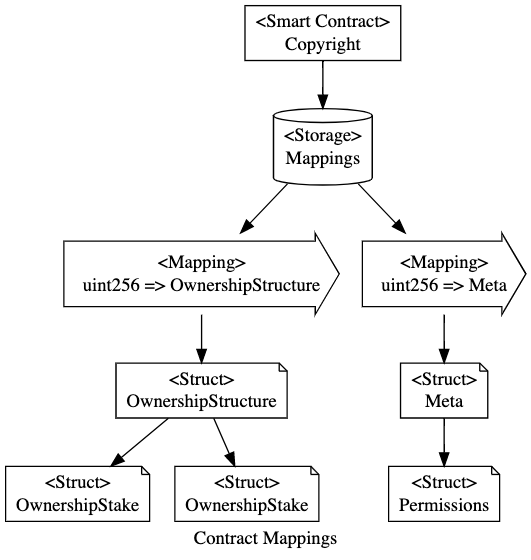
\includegraphics[width=0.5\textwidth,height=0.5\textheight,keepaspectratio]{images/operational/mappings.png}
\label{fig:float}
\end{figure}

To solve this problem I've redesigned how ownership is defined with the smart contract, instead of mapping the token id to one address the contract will now map to an \textbf{OwnershipStructure} which then points to a list of owner addresses along with a number of shares that specific address holds in the token.

This design obviously borrows a lot from limited companies share structure allowing for a complex ownership of multiple individuals or groups with implied variance in ownership (although the number of shares an address owns makes no immediate difference in the current implementation of this contract as this was outside of the desired complexity scope).

\subsubsection{Shareholder consensus}

Allowing multiple wallets to have ownership over a token now introduces a new problem for my contract design, when a change is made everyone has to agree to that change I can't just check if you're an owner anymore, giving the ability to change the copyright to everyone with a stake without consulting with all other owners is a point of exploitation.

\begin{figure}[H]
\caption{Structured Ownership proposal mappings}
\centering
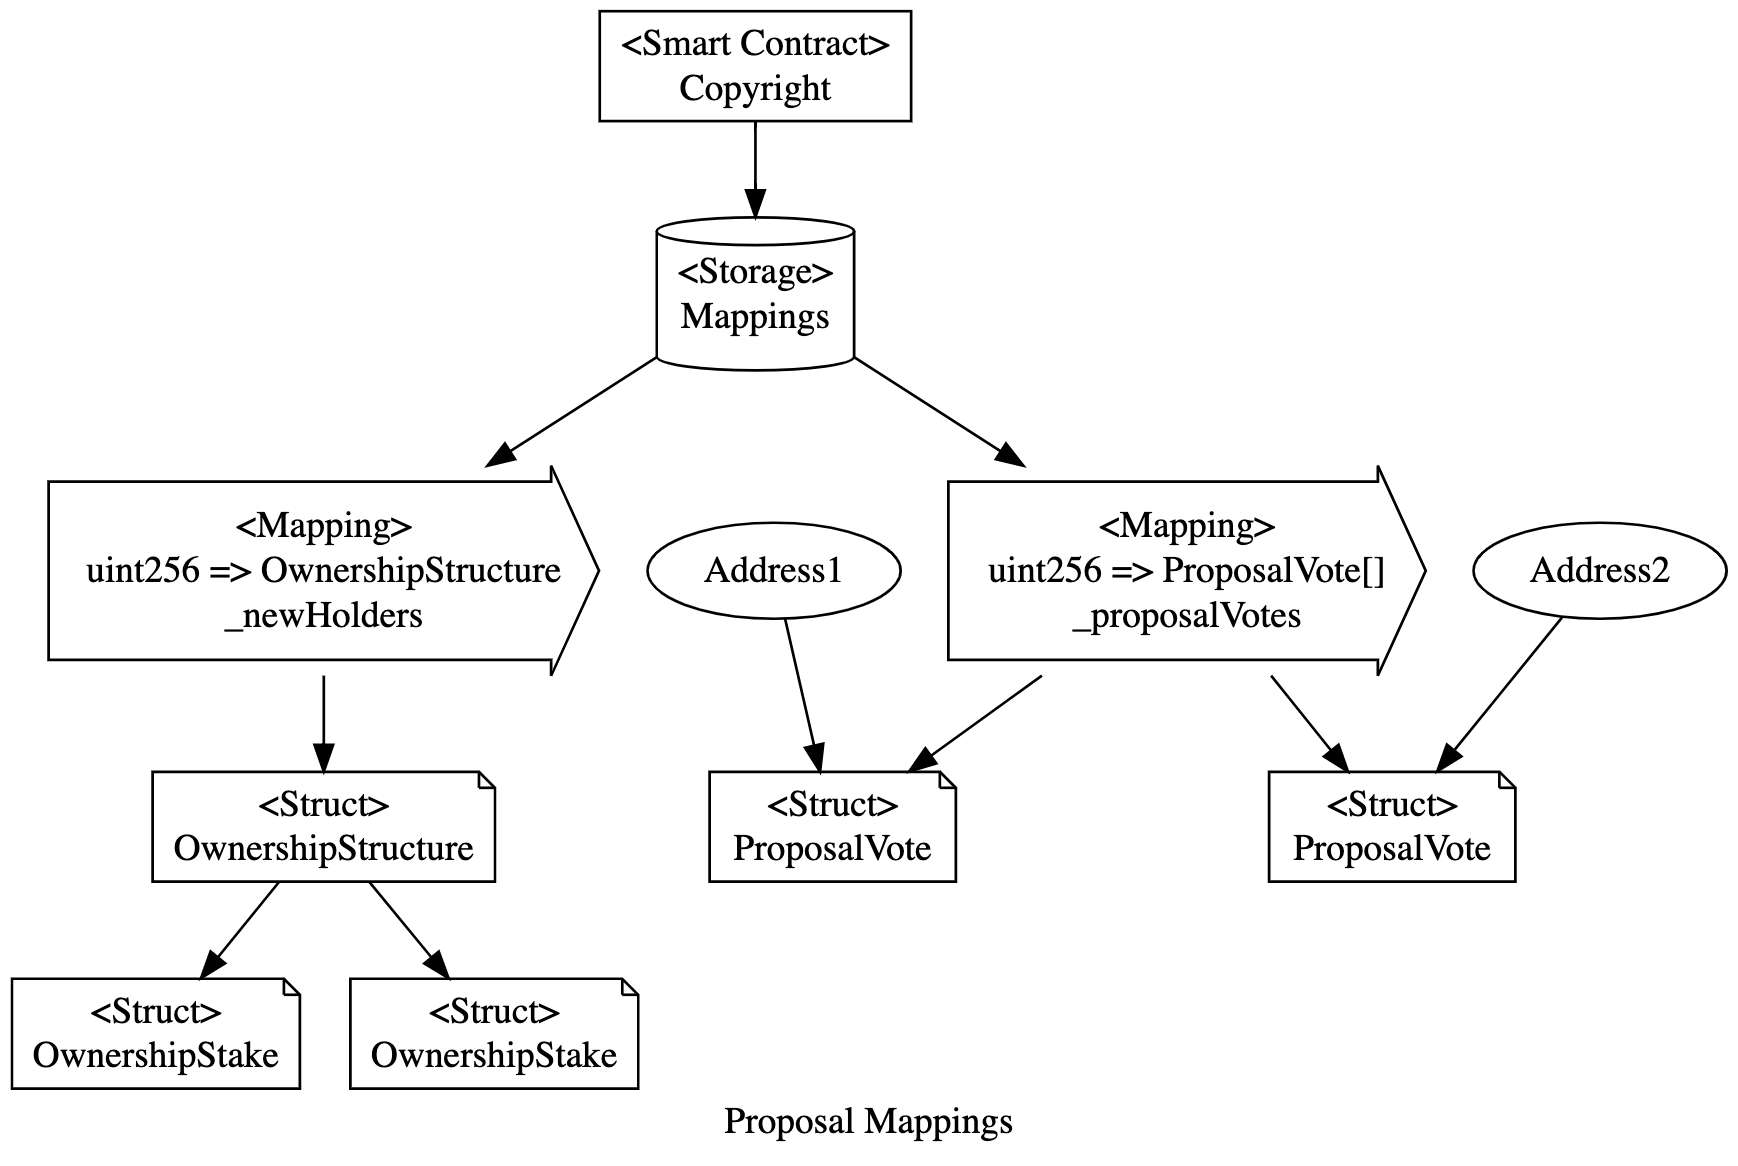
\includegraphics[width=\textwidth,height=\textheight,keepaspectratio]{images/operational/prop-mappings.png}
\end{figure}

This is the solution I've designed for the shareholder consensus problem, now instead of making a direct change to the copyright (in this case an ownership restructure) a user proposes a change to the copyright which is then voted on by all the owners until a unanimous vote tally is reached then the change can be made.

\subsubsection{Permissions/Metadata}

% TODO is this section needed?

\subsection{Back-end}

% TODO some fluff, a mirrored system (blockchain, dotnet)

\subsubsection{Dependancy injection}

% bit iffy could be better?
Dependancy injection is a supported and heavily encouraged design pattern within \textbf{.NET} and \textbf{ASP.NET} which allows for building loosely coupled applications by separating out implementation and design and the ability to depend on a softwares design opposed to its technical implementation allows for more resilient and modular code less dependant on a specific implementation.

\begin{figure}[H]
\caption{DI graph taken from \href{https://docs.microsoft.com/en-us/dotnet/architecture/modern-web-apps-azure/architectural-principles#dependency-inversion}{docs.microsoft}}
\centering
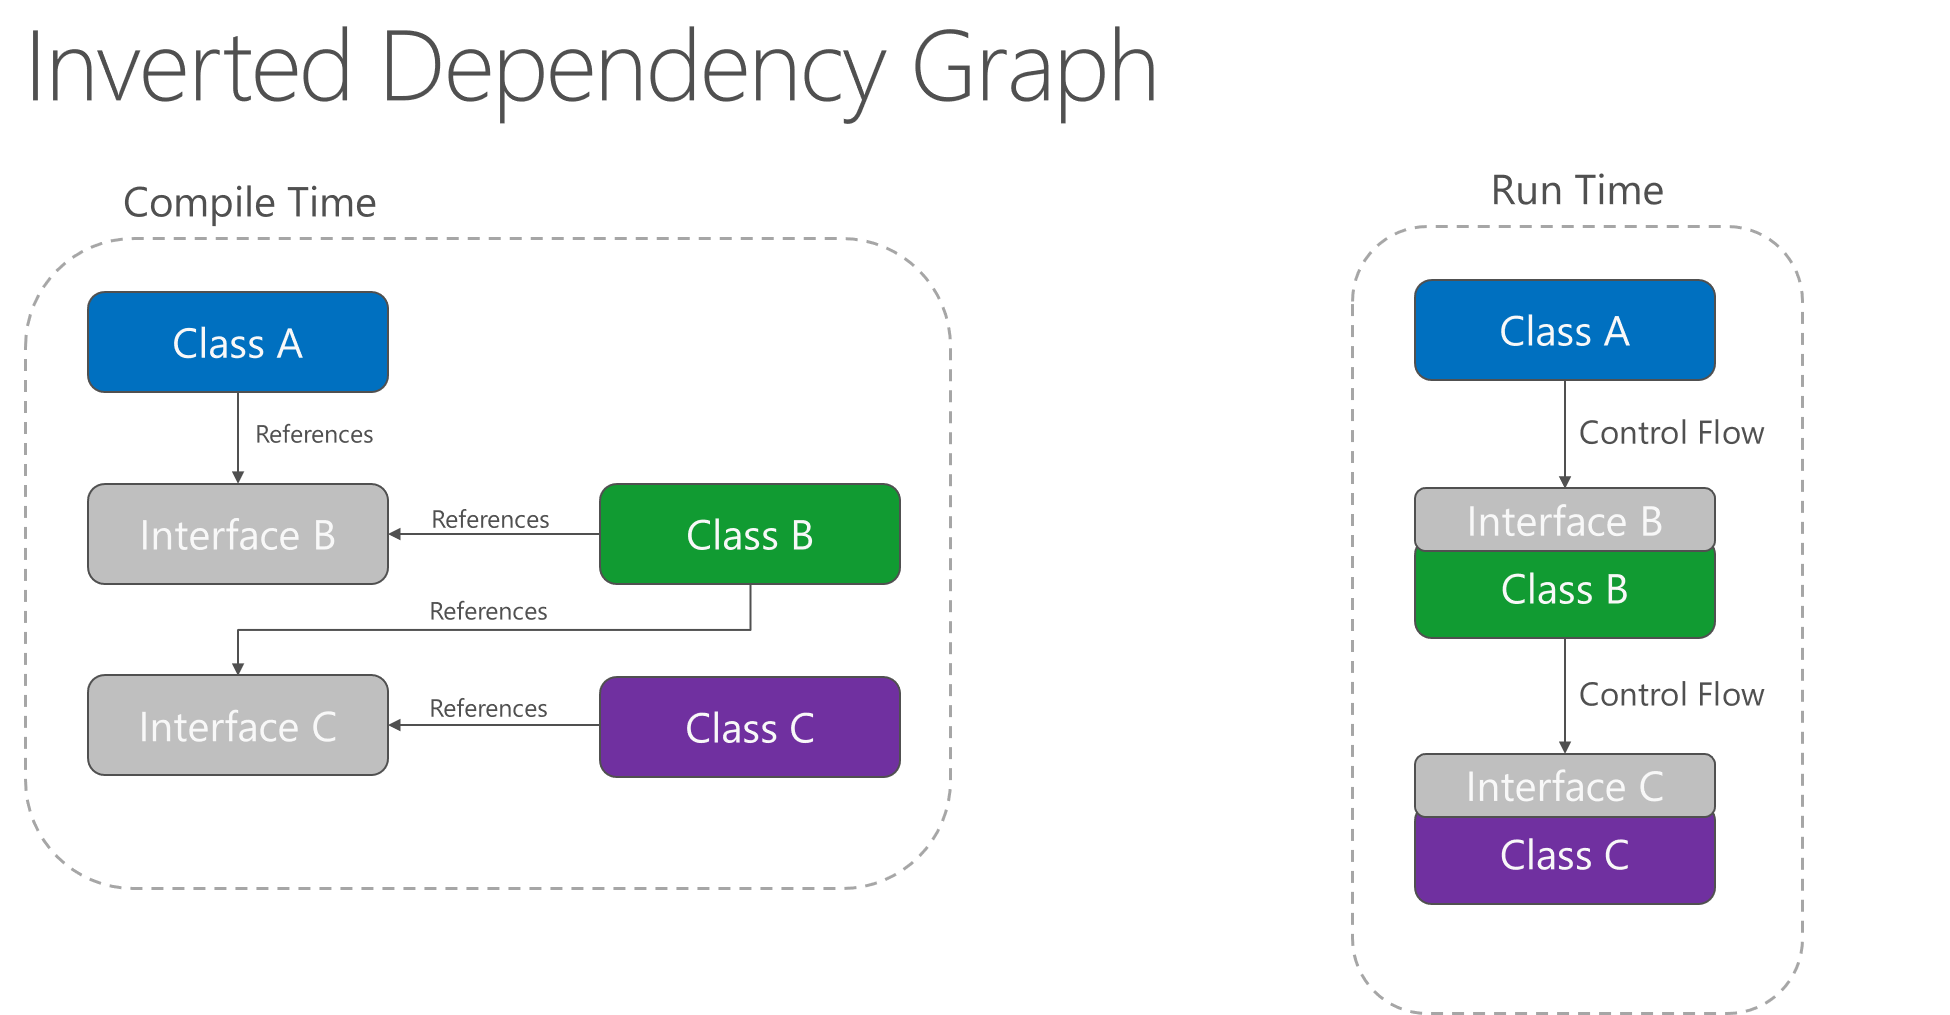
\includegraphics[width=\textwidth,height=\textheight,keepaspectratio]{images/patterns/ms-di}
\centering
\end{figure}

This graph shows a generic example of inversion of control and dependancy injection, as you can see each class is depending on an interface of the desired class not the actual code implementation hence loosely coupled.

\begin{figure}[H]
\caption{Example dependancy graph for the query controller and service}
\centering
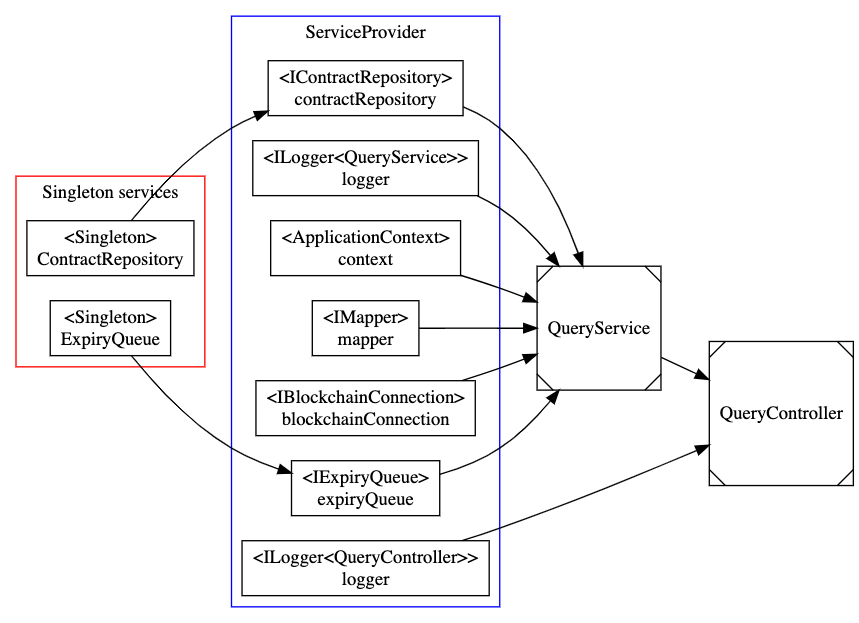
\includegraphics[width=0.7\textwidth,height=0.7\textheight,keepaspectratio]{images/patterns/DI-example}
\end{figure}

This is real example of dependancy injection drawn from the query controller and service injections. It shows that the two classes don't import any other implemented classes just the interfaces describing how you can interact with an implemented version of that class. At run time each interface injected will be populated from the service collection with an implemented version of the class thats be registered on startup.

\subsubsection{Background services}

The design of background services was built on previous work I wrote for \href{https://github.com/mrharrisonbarker/openevent}{OpenEvent} so instead of trying new software like \href{https://www.hangfire.io/}{Hangfire} which does look more feature rich and well used, however I decided for the scale of this project and the already existing pattern I had developed and knew intimately a year ago would be a better fit.

\begin{figure}[H]
\caption{Queued background service pattern}
\centering
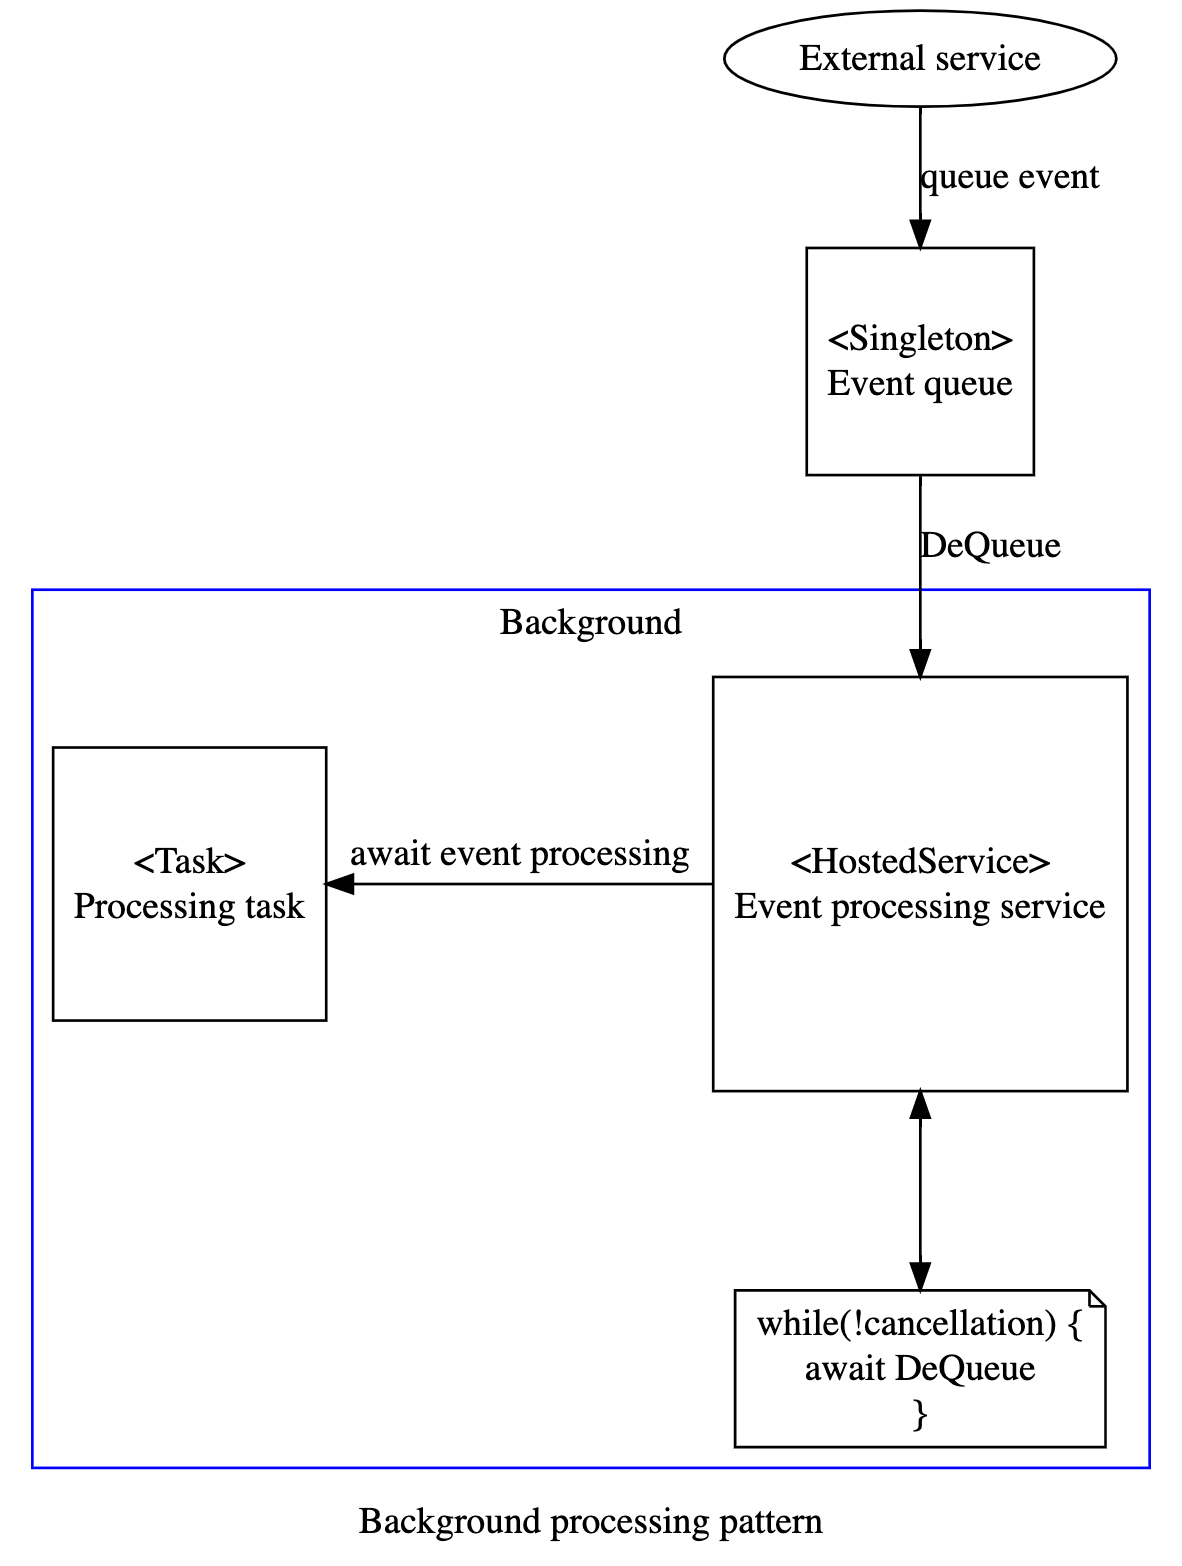
\includegraphics[width=0.5\textwidth,height=0.5\textheight,keepaspectratio]{images/patterns/background-processing-pattern}
\end{figure}

This is the basic design pattern describing how my background services work, it's essentially made up of a queue and processing service. "Work" is queued while a processing service running in its own thread dequeues work then processes accordingly. Once the work has been finished the processing service waits for the next item on the queue.

This pattern can be quickly implemented and tailored to a specific type of background work, it's easily scalable with the number of threads available and settable in the processing service.

\subsubsection{Event processing}

Because transactions on the blockchain can technically take any amount of time to be verified, placed into a block and then for that block to be placed onto the chain. Blocks on \keyword{Ethereum} are processed around every 13 seconds and you're not guaranteed to be placed into the next block which largely depends on the amount of \textbf{gas} you're willing to spend and the number of transactions currently being processed by the network.

All this means that my system has to be able to send a transaction then wait an indeterminate amount of time for a response and I can't force the user to wait on that transaction until complete. Thankfully \keyword{Ethereum} has a solution for this problem called \textbf{Events}, I've specified a number of these events in my contract definition (see below) which the system then "listens" for by processing the information in each block.

\begin{figure}[H]
\caption{\href{https://github.com/MrHarrisonBarker/CRPL/blob/main/CRPL.Contracts/contracts/IStructuredOwnership.sol}{IStructuredOwnership} events}
\begin{lstlisting}[language=Solidity]
/// @dev Emits when a new copyright is registered
event Registered(uint256 indexed rightId, OwnershipStake[] to);

/// @dev Emits when a copyright has been restructured and bound
event Restructured(uint256 indexed rightId, RestructureProposal proposal);

/// @dev Emits when a restructure is proposed
event ProposedRestructure(uint256 indexed rightId, RestructureProposal proposal);

/// @dev Emits when a restructure vote fails
event FailedProposal(uint256 indexed rightId);
\end{lstlisting}
\end{figure}

When an event is found it gets added to a processing queue then a processing service dequeues each event and processes based on the type of event (this uses the background service pattern discussed in the previous section).

\begin{figure}[H]
\caption{Blockchain event listeners and processing}
\centering
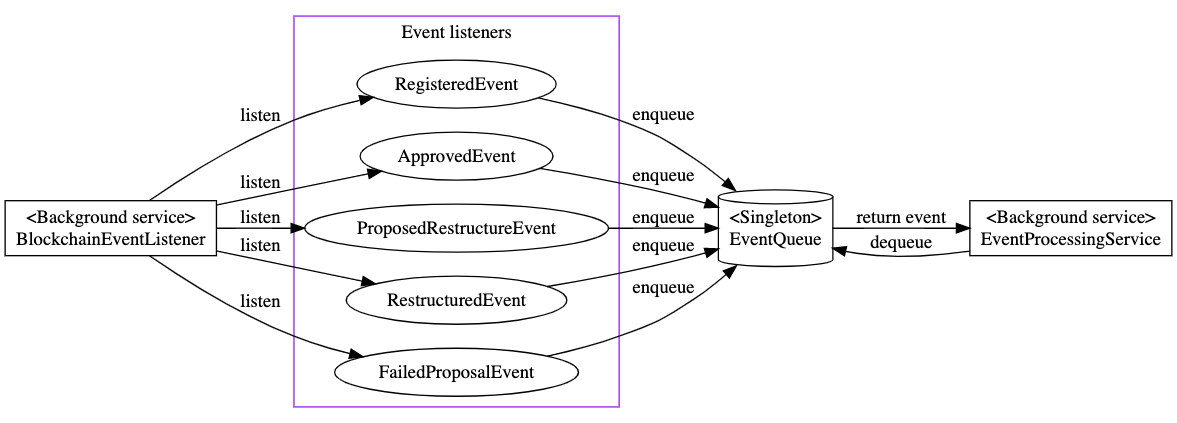
\includegraphics[width=\textwidth,height=0.5\textheight,keepaspectratio]{images/operational/Event-Listening}
\end{figure}

\subsubsection{Applications framework}
% TODO Data model structure (application, view model, input model)

Handling forms and applications is awkward and full of edge cases, the code for handing these applications (eg: copyright registration) can become large and convoluted especially when your system implements many. For this system five applications are needed: copyright registration, ownership restructure, dispute, wallet transfer and delete account. I decided to design a solution for handling application flow and state as a generic process, this means all applications will follow the same state flow and interaction endpoints \textit{seen below.} 

\begin{figure}[H]
\caption{Applications framework state diagram}
\centering
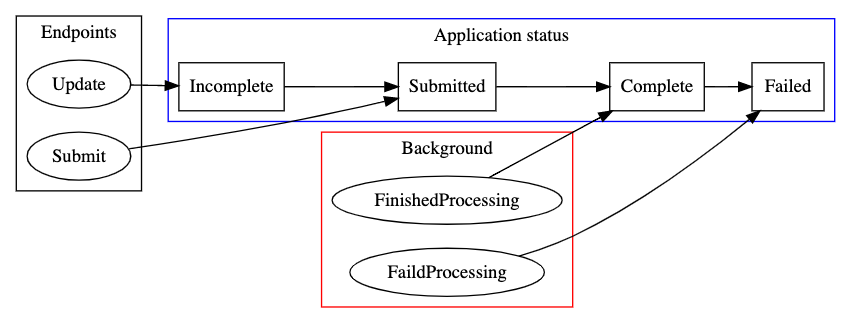
\includegraphics[width=\textwidth,height=0.5\textheight,keepaspectratio]{images/operational/applications-status}
\end{figure}

This generification and ridged design flow proved extremely useful, this was because keeping a clear view of state is essential when keeping parity between my system and the outer \keyword{blockchain}.

\subsection{Database}

The database for this system needs to store two types of data: data stored on both the \keyword{blockchain} and CRPL (eg: public wallet addresses, contract address, and registered works) and data stored solely on the database not mirrored with the chain (eg: applications, user account information and explicit database relationships).

\begin{figure}[H]
\caption{Database EER diagram}
\centering
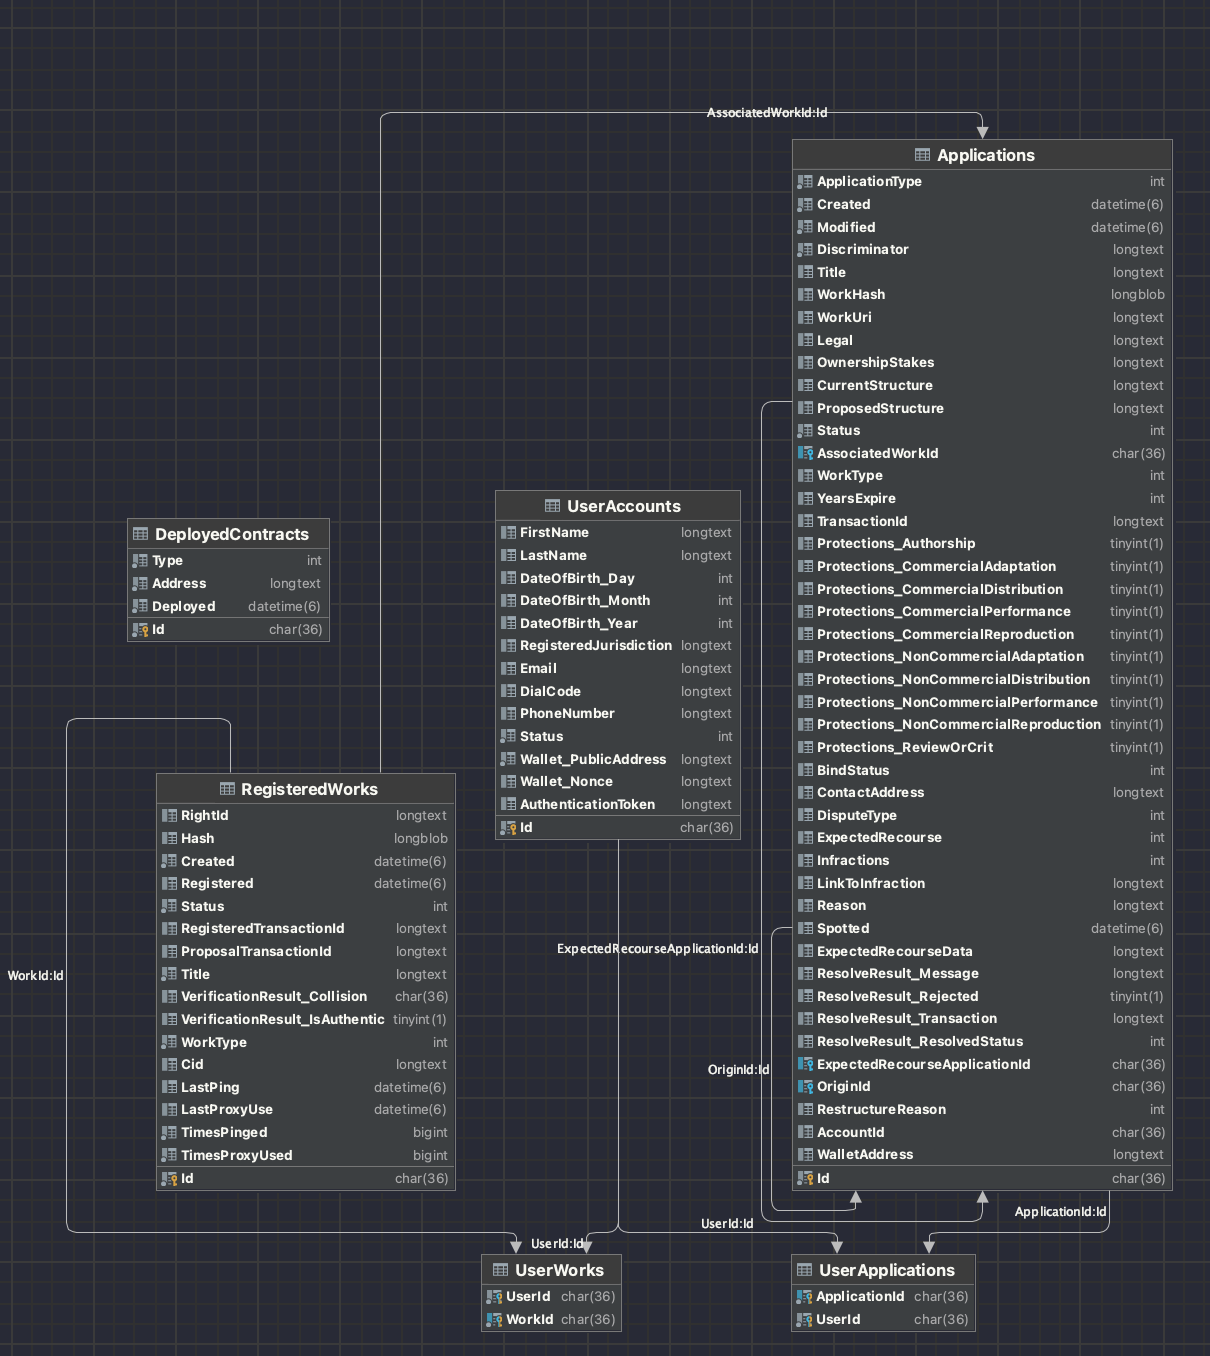
\includegraphics[width=\textwidth,height=0.7\textheight,keepaspectratio]{images/patterns/database}
\end{figure}

\subsubsection{Chain parity}

Data need to be kept in parity with the \keyword{blockchain} introduces a problem that being data on the chain can change independently of the system, a user could transact with the \keyword{copyright} \keyword{smart contract} and register a new copyright or propose a new ownership structure and even bind that new structure completely destroying any continuity between my database and what's real. This will lead to a terrible user experience but there's nothing I can do about it, the chain is open to anyone and is quite literally the whole point of this project.

However I can react to change, again everything is open and accessible all I have to do is read the \keyword{blockchain} and update my database accordingly keeping in mind that the chain is always the one source of truth not my database.

\subsubsection{Independent from the chain}

I've chosen to keep certain data off the \keyword{blockchain} only representing it on the CRPL database. Of course technically I could store everything on chain completely independent of any database, however this would ballon the size of my \keyword{smart contract} which are limited to 24KB complied it would also create a problem for maintainability and future development. 
Imagine everything is represented in the smart contract including dispute handling and applications, the contract is verified onto the chain and is now running in the \keyword{EVM} what happens when I want to add a new type of application or I find out my dispute handling is un-ethical or exploitable? I can't change the smart contract its immutable if I really wanted to I could deploy a new contract and manually migrate all previous \keyword{copyrights} to this new contract, however this would be expensive, slow and arguably against the spirit of \keyword{blockchain} technology and the law as I'm effectively changing the underlying representation of a users \keyword{copyright} without their consultation or approval.

\subsection{Front-end}
% TODO form design and working

Visual design of the web application was on the lowest priority a focus on pure usability and function was always the priority because of the complex undertaking that was needed to implement all functionality building effectively two backend systems (\keyword{blockchain} and web API).

I decided to use the \href{https://clarity.design/}{Clarity} design system and libraries as they have support for Angular and has an enterprise/function first focus.

\begin{figure}[H]
\caption{Original dashboard page wireframe}
\centering
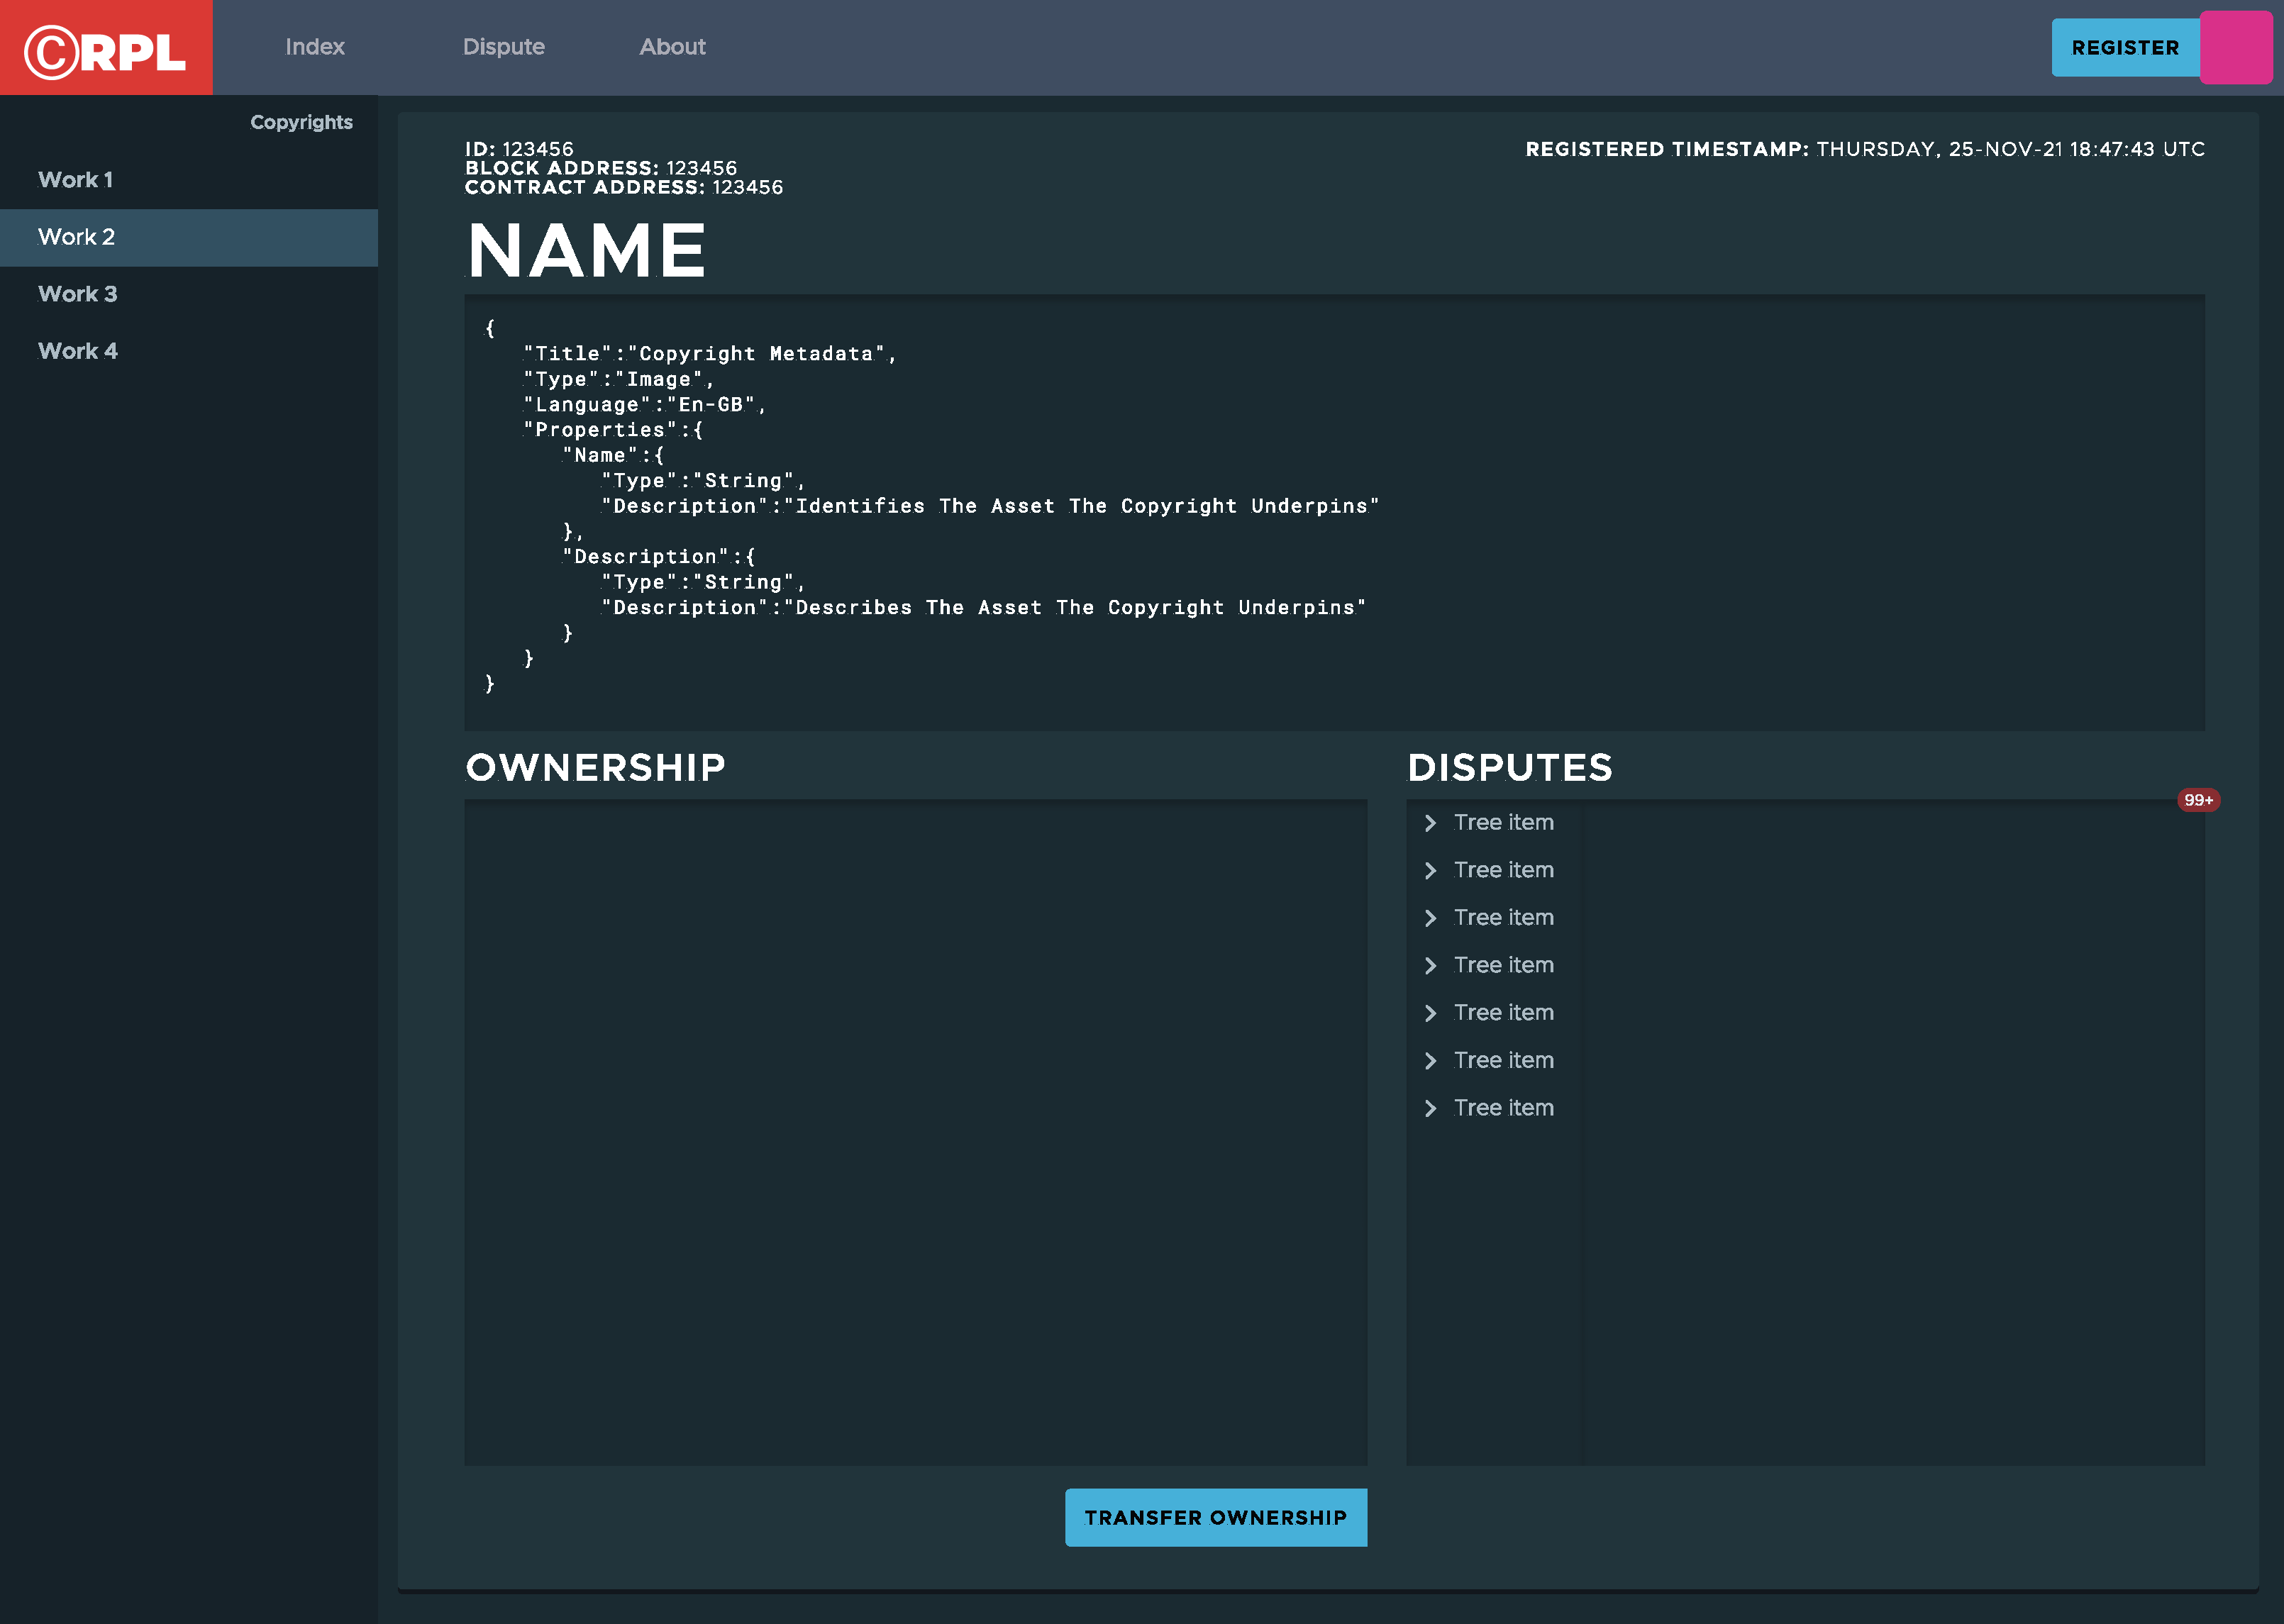
\includegraphics[width=\textwidth,height=0.5\textheight,keepaspectratio]{images/wireframe/Dashboard}
\end{figure}

\begin{figure}[H]
\caption{Final dashboard design}
\centering
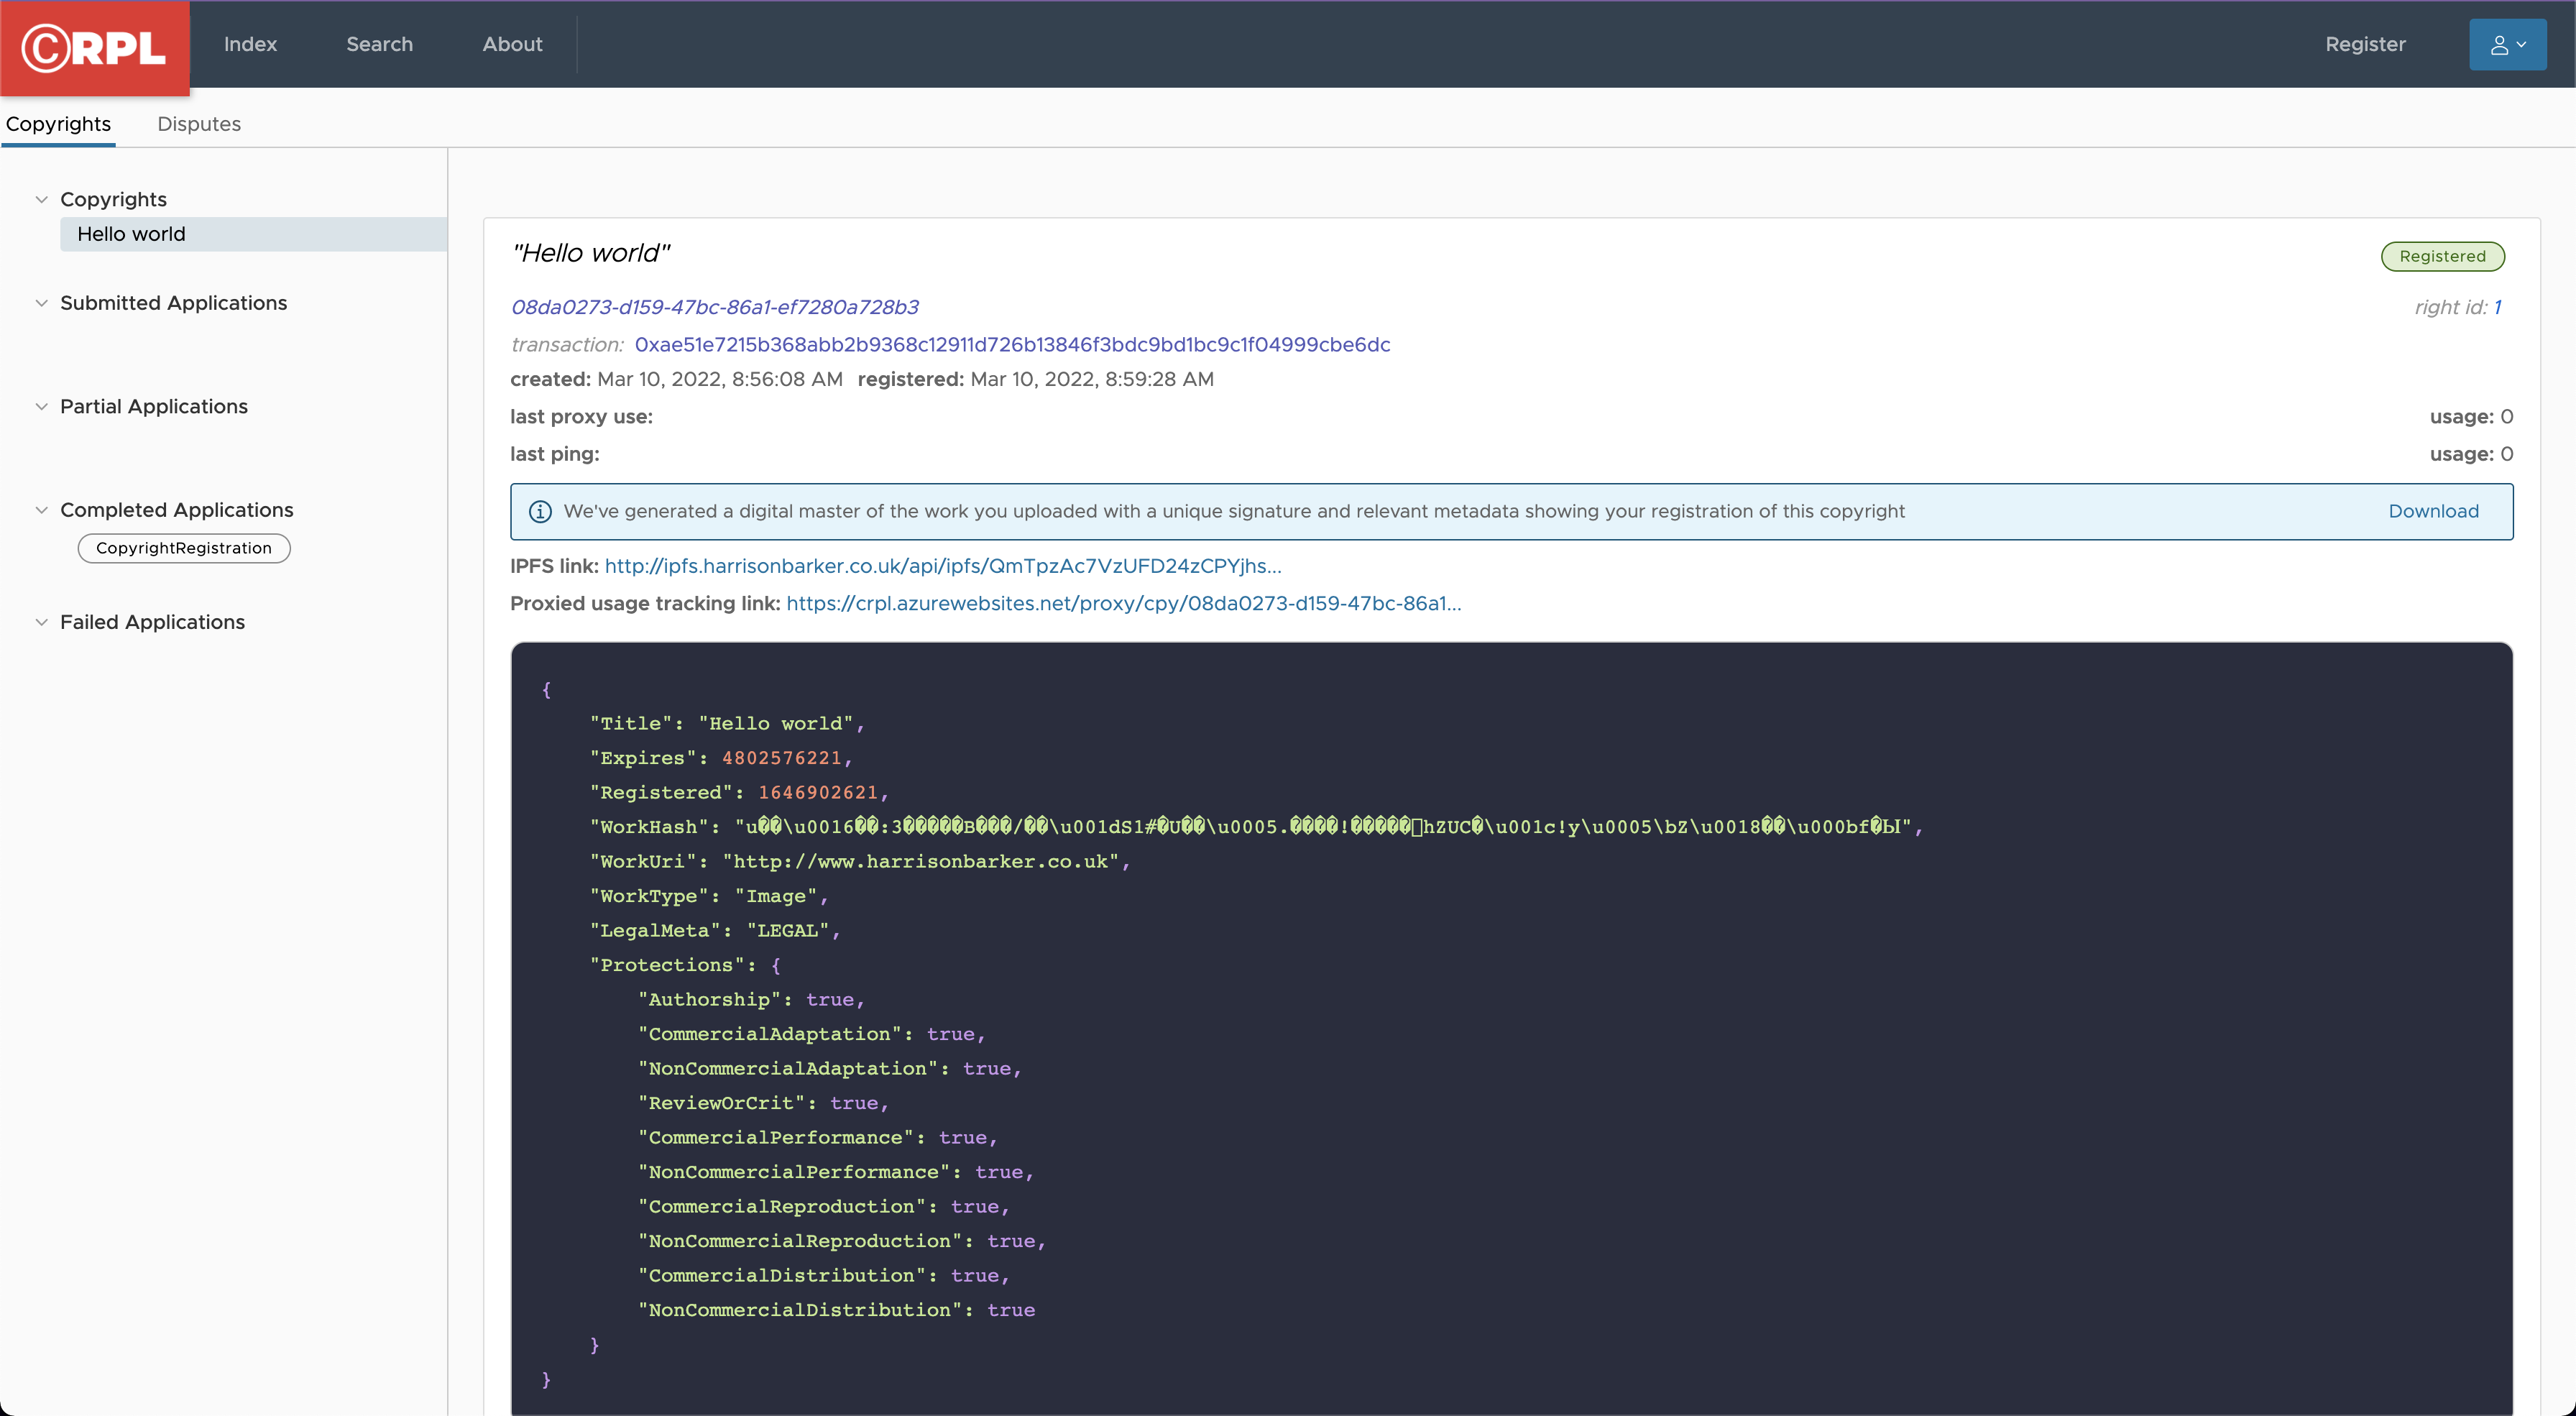
\includegraphics[width=\textwidth,height=0.5\textheight,keepaspectratio]{images/wireframe/dashboard-real}
\end{figure}

\begin{figure}[H]
\caption{Original register form wireframe}
\centering
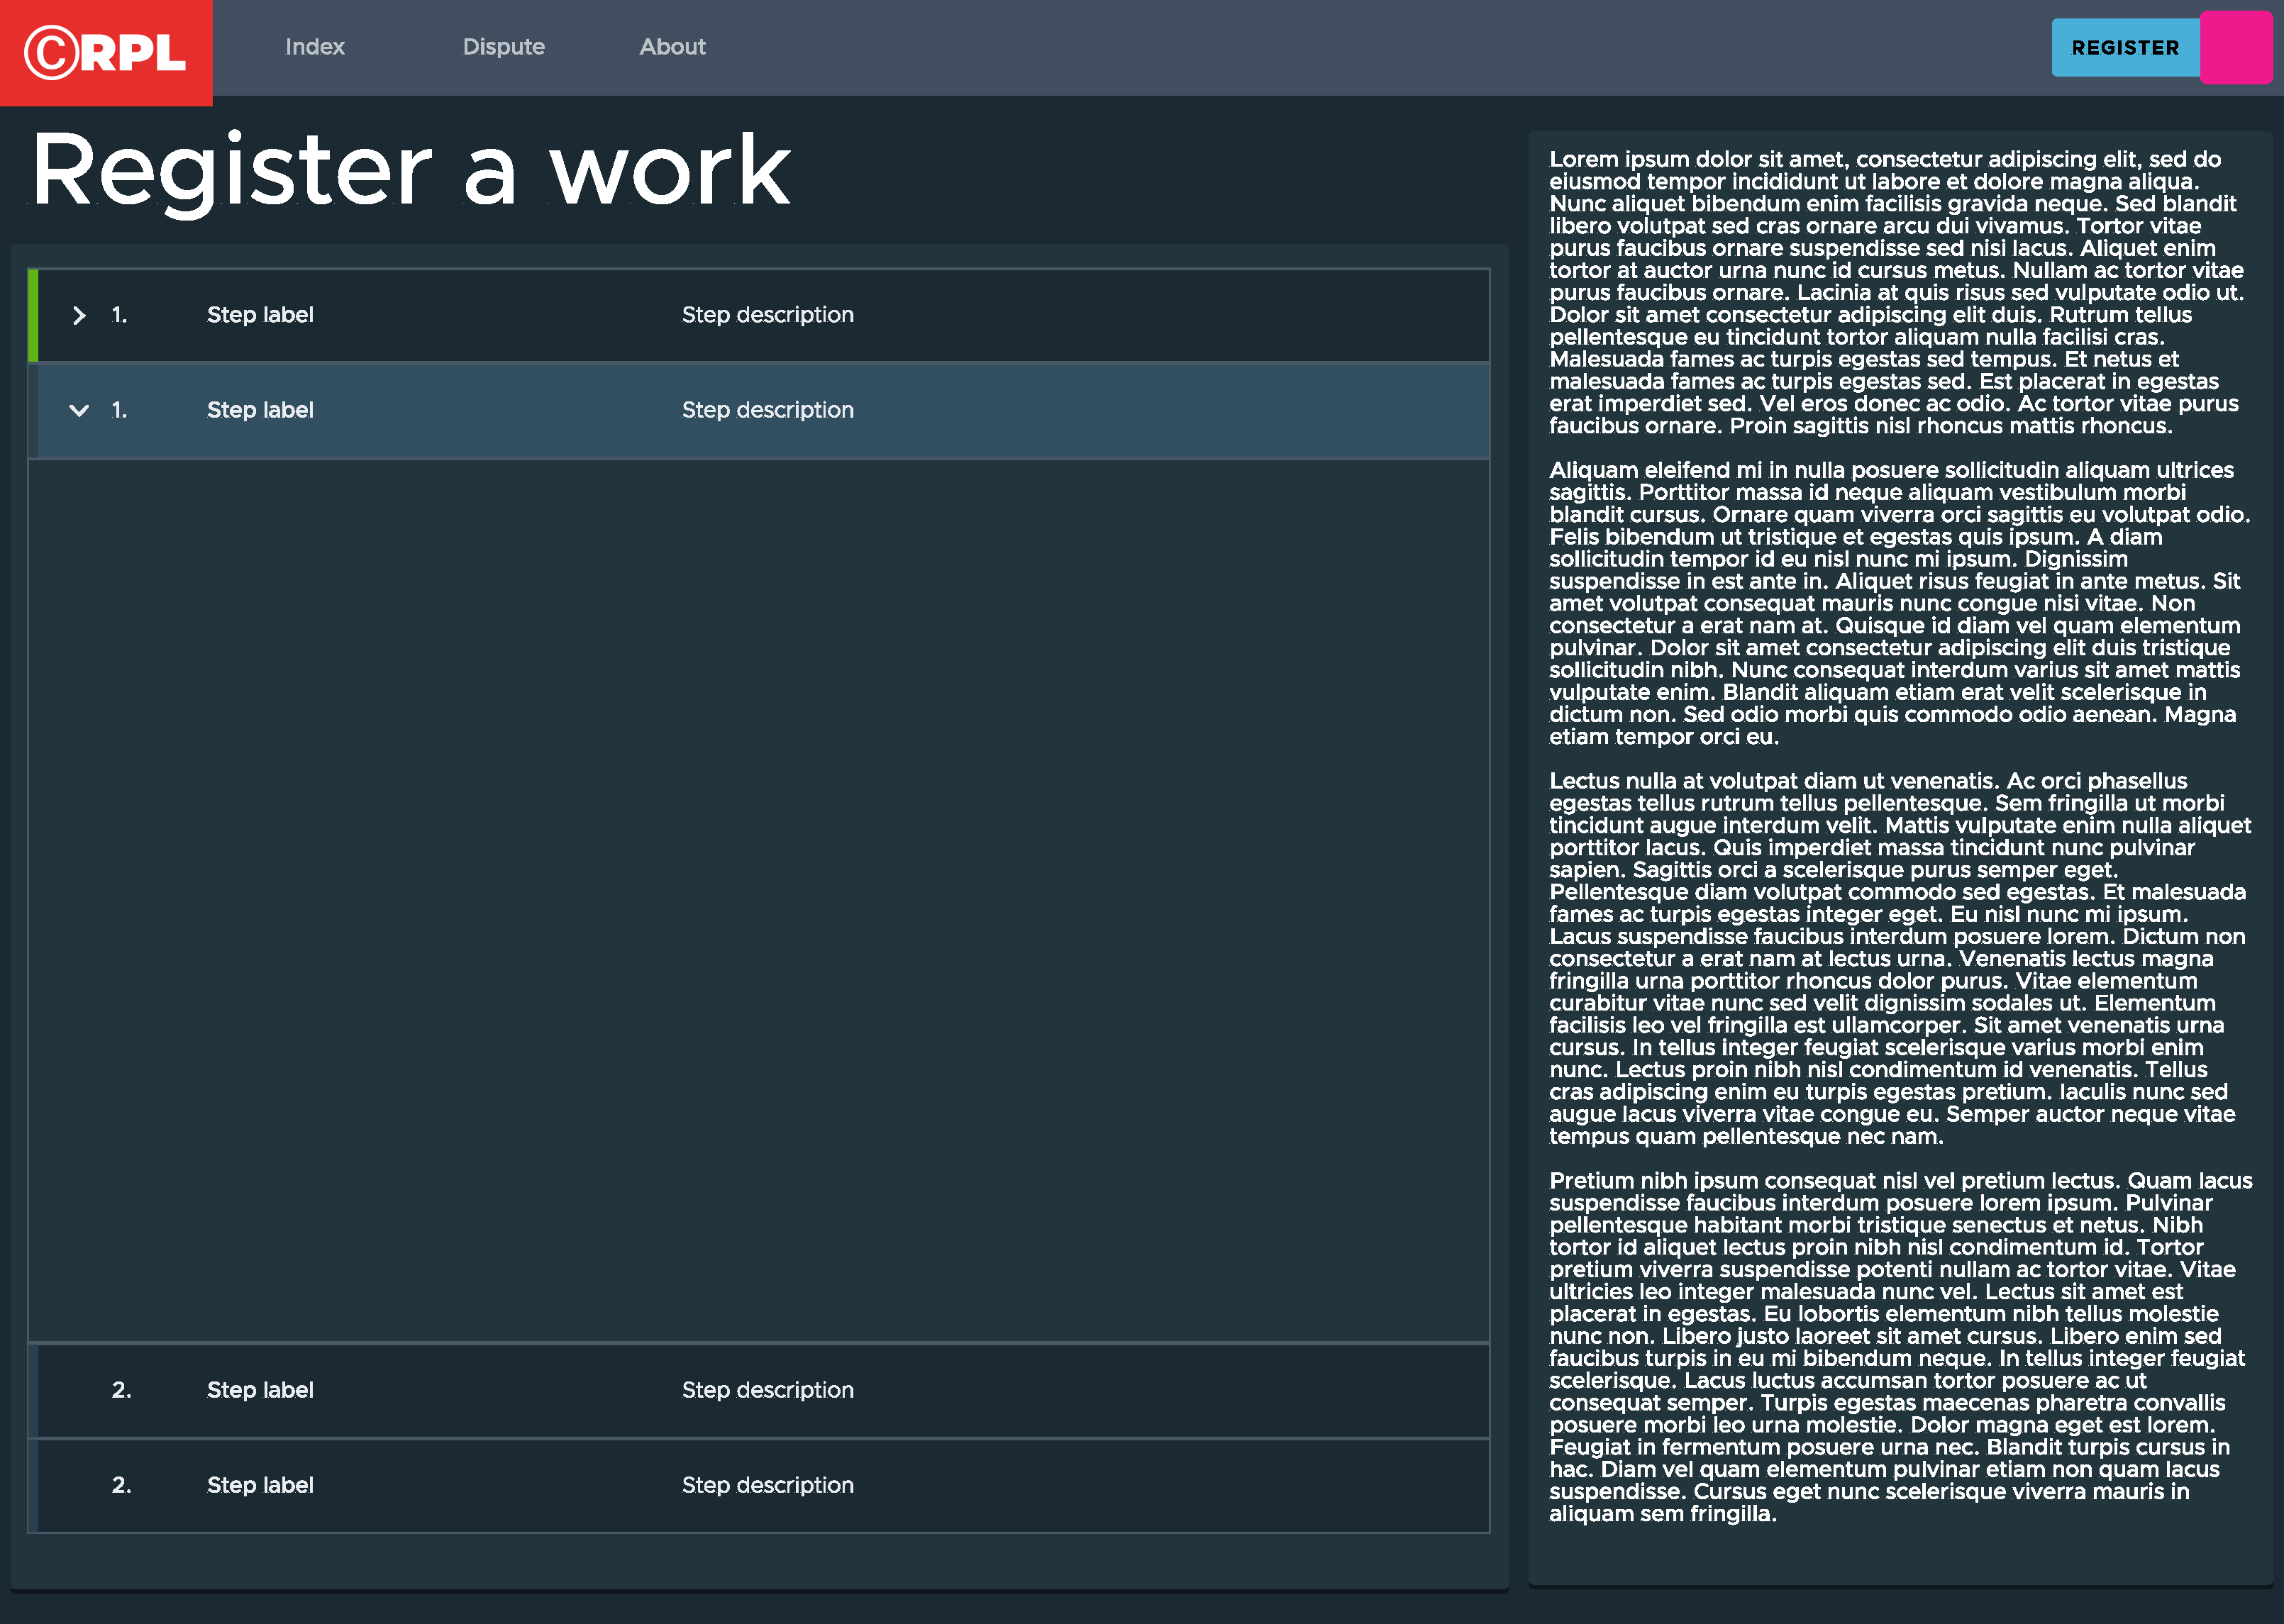
\includegraphics[width=\textwidth,height=0.5\textheight,keepaspectratio]{images/wireframe/Register}
\end{figure}

\begin{figure}[H]
\caption{Final register design}
\centering
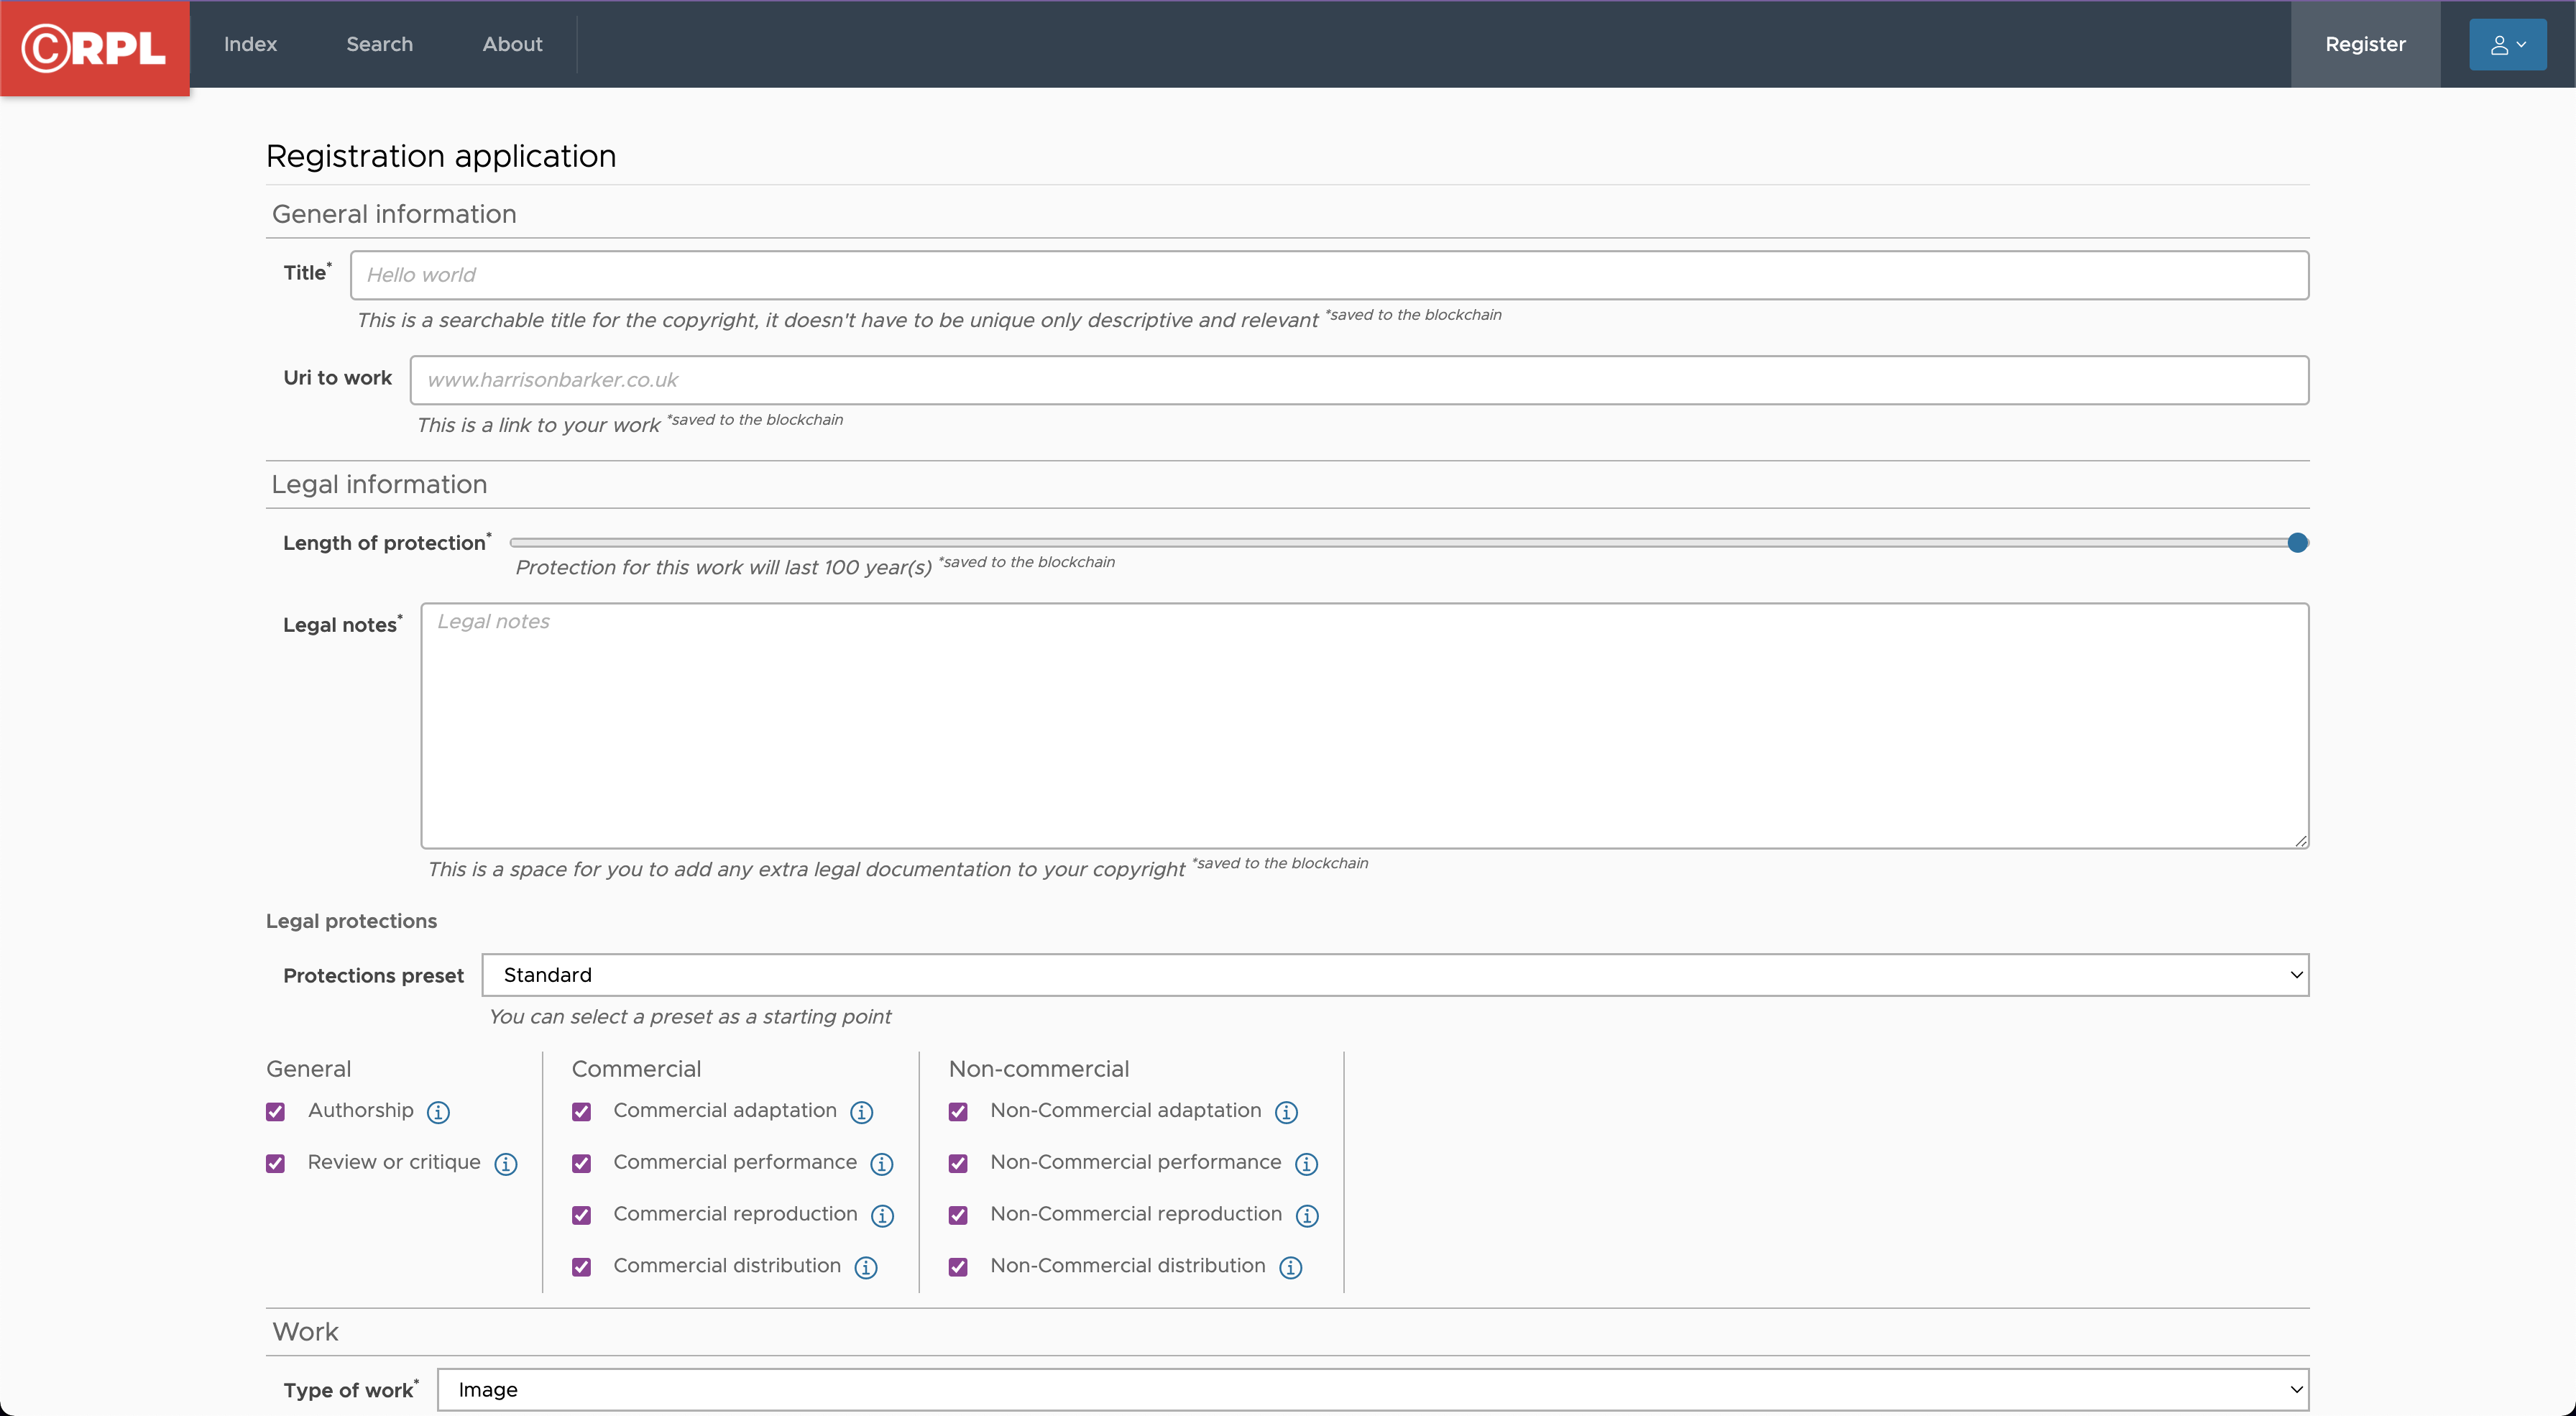
\includegraphics[width=\textwidth,height=0.5\textheight,keepaspectratio]{images/wireframe/register-real}
\end{figure}

\subsection{Architecture}
% TODO an overview of the system architecture design

\subsection{Development process}

Development was split into four sprints, two larger sprints two weeks long to start development focusing on major core features essential for any success of the project: \keyword{smart contracts}, contract interaction, registration and restructure applications and user authentication. Followed up with two one week sprints focusing on secondary features and quality of life: disputes, search, synchronisation and account config. 

\begin{figure}[H]
\hfil
\begin{tabular}{|l|l|l|l|}
\hline
Sprint & Start            & End              & Length  \\ \hline
1      & 19 January 2022  & 2 February 2022  & 2 weeks \\ \hline
2      & 4 February 2022  & 18 February 2022 & 2 weeks \\ \hline
3      & 20 February 2022 & 27 February 2022 & 1 week  \\ \hline
4      & 1 March 2022     & 8 March 2022     & 1 week  \\ \hline
\end{tabular}
\end{figure}

\section{Implementation}

\subsection{Smart contract}
% TODO saved metadata

\subsubsection{Interface overview}

% TODO this is a bit weak

The contract interface is split into two, \href{https://github.com/MrHarrisonBarker/CRPL/blob/main/CRPL.Contracts/contracts/IStructuredOwnership.sol}{IStructuredOwnership.sol} which handles multi-ownership transactions and events and \href{https://github.com/MrHarrisonBarker/CRPL/blob/main/CRPL.Contracts/contracts/ICopyright.sol}{ICopyright.sol} which handles all \keyword{copyright} transactions and events (similar to the \href{https://eips.ethereum.org/EIPS/eip-721}{EIP-721} interface).

\begin{figure}[H]
\caption{ICopyright events}
\begin{lstlisting}[language=Solidity]
/// @dev Emits when a new address is approved to a copyright
event Approved(uint256 indexed rightId, address indexed approved);

/// @dev Emits when a new manager has been approved
event ApprovedManager(address indexed owner, address indexed manager, bool hasApproval);
\end{lstlisting}
\end{figure}

\begin{figure}[H]
\caption{IStructuredOwnership events}
\centering
\begin{lstlisting}[language=Solidity]
/// @dev Emits when a new copyright is registered
event Registered(uint256 indexed rightId, OwnershipStake[] to);

/// @dev Emits when a copyright has been restructured and bound
event Restructured(uint256 indexed rightId, RestructureProposal proposal);

/// @dev Emits when a restructure is proposed
event ProposedRestructure(uint256 indexed rightId, RestructureProposal proposal);

/// @dev Emits when a restructure vote fails
event FailedProposal(uint256 indexed rightId);
\end{lstlisting}
\end{figure}

If we first look at all the events defined most are simply explained and straight forward, \textit{Approved} and \textit{ApproveManager} are taken from the \nft standard (ApproveManager == ApprovalForAll) then for IStructuredOwnership I've introduced four new events enabling modifiable multi address ownership with consensus.


\begin{figure}[H]
\caption{IStructuredOwnership functions}
\centering
\begin{lstlisting}[language=Solidity]
/// @notice The current ownership structure of a copyright
/// @param rightId The copyright id
function OwnershipOf(uint256 rightId) external view returns (OwnershipStake[] memory);

/// @notice Proposes a restructure of the ownership share of a copyright contract, this change must be bound by all share holders
/// @param rightId The copyright id
/// @param restructured The new ownership shares
/// @param notes Any notes written concerning restructure for public record
function ProposeRestructure(uint256 rightId, OwnershipStake[] memory restructured) external payable;

/// @notice The current restructure proposal for a copyright
/// @param rightId The copyright id
/// @return A restructure proposal
function Proposal(uint256 rightId) external view returns (RestructureProposal memory);
    
function CurrentVotes(uint256 rightId) external view returns (ProposalVote[] memory);

/// @notice Binds a shareholders vote to a restructure
/// @param rightId The copyright id
/// @param accepted If the shareholder accepts the restructure
function BindRestructure(uint256 rightId, bool accepted) external payable;
\end{lstlisting}
\end{figure}

Then the four new and one modified functions to enable this functionality, \textit{ProposeRestructure} to propose a change of ownership and \textit{BindRestructure} to vote and come to consensus between the shareholders. \textit{OwnershipOf} is modified from \textit{ownerOf} from \nft which returns an address but now has to return a complex ownership structure.

\subsubsection{Registration}
% TODO how each copyright is saved (maximum size?)

Registration of a \keyword{copyright} as discussed in the \textit{Smart contract design} section uses the basic principles of existing contract implementations most importantly the \nft contract, which registers new tokens by assigning a wallet address as the result of a token's id in a mapping (hash table) stored on the contract. This is simple and secure as the resulting hash of a token id will always point to the same entry in the mapping and therefore address.

\begin{figure}[H]
\caption{Essential copyright mappings from \href{https://github.com/MrHarrisonBarker/CRPL/blob/main/CRPL.Contracts/contracts/Copyrights/CopyrightBase.sol}{CopyrightBase.sol}}
\centering
\begin{lstlisting}[language=Solidity]
// rightId -> ownership structures
mapping (uint256 => OwnershipStructure) internal _shareholders;
    
// rightId -> metadata
mapping(uint256 => Meta) internal _metadata;
\end{lstlisting}
\end{figure}

I've taken this design and modified it for my needs by mapping to a complex ownership structure instead of one address (enabling multi-ownership), I've then added a new mapping to save metadata (work hash, expiry date, legal protections) for each \keyword{copyright}. These technically could be merged into one mapping along with the four others, mapping from id to a larger more complex struct encompassing all data needed. However I wanted to keep the size of my data structures small with their own defined purpose, this also reduces transaction costs because only the data relevant is being processed.

\begin{figure}[H]
\caption{Register function from \href{https://github.com/MrHarrisonBarker/CRPL/blob/main/CRPL.Contracts/contracts/Copyrights/CopyrightBase.sol}{CopyrightBase.sol}}
\centering
\begin{lstlisting}[language=Solidity]
function Register(OwnershipStake[] memory to, Meta memory meta) public validShareholders(to) {
	
	uint256 rightId = _copyCount.next();

	// registering copyright across all shareholders
	for (uint256 i = 0; i < to.length; i++) {

		require(to[i].share > 0, INVALID_SHARE);

		_recordRight(to[i].owner);
		_shareholders[rightId].stakes.push(to[i]);
	}
        
	_metadata[rightId] = meta;
	_shareholders[rightId].exists = true;
        
	_approvedAddress[_copyCount.getCurrent()] = msg.sender;

	emit Registered(rightId, to);
	emit Approved(rightId, msg.sender);
}	
\end{lstlisting}
\end{figure}

As you can see from the above registration is straightforward: generate the next id, iterate over all shareholders inputted, add each shareholder to the mapping checking each has some shares, add metadata to mapping, approve the sender for this \keyword{copyright} and emit a registered and approved event to let my system know whats happened.

Lastly I want to focus on line 8, \textit{require} is apart of \textbf{Solidity}'s error handling. The \keyword{EVM} runs all functions transactionally in the programming sense meaning all changes to the persistent data structure are processed and saved after the function has completed successfully. This is extremely useful and greatly simplifies error handling because if we encounter an error no underlying changes to the data have taken place and the transaction simply fails. 

\textit{Require} therefore simply checks an expression is true and if not an error is thrown with a stated reason the transaction is canceled and no changes to any stored data structure are made. These are used throughout my \keyword{smart contract} to validate input data, I talk more about these in the \textit{Modifiers} section below. This \textit{require} on line 8 is checking all shareholders have more than zero shares otherwise throw and error with the reason "INVALID\_SHARE".

The events emitted from this function are "listened" to and processed in the back-end more information in the \textit{Blockchain event listeners} section below.

\subsubsection{Ownership restructure}

As discussed in the design of my \keyword{smart contract} I had to build a shareholder consensus function for making changes to the \keyword{copyright}, therefore changing the ownership structure is split into two functions/steps, first you propose a new structure then each shareholder must vote or \textit{"bind"} the new structure, when all the shareholders have agreed to the new structure mappings are updated to reflect the new ownership.

\begin{figure}[H]
\caption{ProposeRestructure function from \href{https://github.com/MrHarrisonBarker/CRPL/blob/main/CRPL.Contracts/contracts/Copyrights/CopyrightBase.sol}{CopyrightBase.sol}}
\centering
\begin{lstlisting}[language=Solidity]
function ProposeRestructure(uint256 rightId, OwnershipStake[] memory restructured) external override validId(rightId) isExpired(rightId) validShareholders(restructured) isShareholderOrApproved(rightId, msg.sender) payable {
        
        for (uint256 i = 0; i < restructured.length; i++) {

            require(restructured[i].share > 0, INVALID_SHARE);

            _newHolders[rightId].stakes.push(restructured[i]);
            _newHolders[rightId].exists = true;
        }   

        emit ProposedRestructure(rightId, _getProposedRestructure(rightId));
    }	
\end{lstlisting}
\end{figure}

Above is the first step of restructuring the proposal, this is a small function that simply iterates through all the new shareholders and added their address and shares to a new mapping called \textit{\_newHolders} which is the same as the \textit{\_shareholders} mapping and is there to hold proposed ownership structures before they're "bound". An event is emitted which tells the back-end that the proposal has been saved to the chain and to start accepting votes from owners.

\begin{figure}[H]
\caption{BindRestructure function from \href{https://github.com/MrHarrisonBarker/CRPL/blob/main/CRPL.Contracts/contracts/Copyrights/CopyrightBase.sol}{CopyrightBase.sol}}
\centering
\begin{lstlisting}[language=Solidity]
function BindRestructure(uint256 rightId, bool accepted) external override validId(rightId) isExpired(rightId) isShareholderOrApproved(rightId, msg.sender) payable 
{
	_checkHasVoted(rightId, msg.sender);
     
	// record vote
	_proposalVotes[rightId].push(ProposalVote(msg.sender, accepted));
	_numOfPropVotes[rightId] ++;

	for (uint256 i = 0; i < _proposalVotes[rightId].length; i ++) 
	{
		if (!_proposalVotes[rightId][i].accepted) 
		{
			_resetProposal(rightId);
			emit FailedProposal(rightId);

			return;
		}
	}

	// if the proposal has enough votes, **** 100% SHAREHOLDER CONSENSUS ****
	if (_numOfPropVotes[rightId] == _numberOfShareholder(rightId)) {
            
		// proposal has been accepted and is now binding

		OwnershipStake[] memory oldOwnership = OwnershipOf(rightId);
            
		// reset has to happen before new shareholders are registered to remove data concerning old shareholders
		_resetProposal(rightId);

		_shareholders[rightId] = _newHolders[rightId];

		delete(_newHolders[rightId]);

		emit Restructured(rightId, RestructureProposal({oldStructure: oldOwnership, newStructure: OwnershipOf(rightId)}));
	}
}	
\end{lstlisting}
\end{figure}

Now looking at the more complex \textit{BindRestructure} function: first the address is checked if they've voted already, the vote is then recorded in a new mapping \textit{\_proposalVotes}, all votes are checked, if any of the votes are false then the whole proposal is rejected, checks if all the shareholders have voted, if all the votes are in set \textit{\_shareholders} to the proposed structure from \textit{\_newHolders} and emit an event.
\br
This is a point of possible future development or discussion, for a proposal to be \textit{"bound"} a unanimous vote is needed however this system could take advantage of the distribution of shares with only a majority of shares needed to make a change.

I decided to keep the voting unanimous over concerns of complexity (extension of development time was predicted) and a possible moral issues as to the possibilities of exploitation using this. An issue of exploitation is inherent to both implementations however a unanimous vote gives equal power of exploitation to every party whereas using shares would give more power to high staked parties.
 

\subsubsection{Modifiers}

Modifiers are pieces of code run at either end of a function call usually used to verify function parameters, I'm using them exclusively at the start of function calls to test addresses, ids and expiry. The design of a modifier usually consists of an assertion plus any processing needed on the data. 

\begin{figure}[H]
\caption{isShareholderOrApproved modifier from \href{https://github.com/MrHarrisonBarker/CRPL/blob/main/CRPL.Contracts/contracts/Copyrights/CopyrightBase.sol}{CopyrightBase.sol}}
\centering
\begin{lstlisting}[language=Solidity]
modifier isShareholderOrApproved(uint256 rightId, address addr) 
{
	uint256 c = 0;
	for (uint256 i = 0; i < _shareholders[rightId].stakes.length; i++) 
	{
		if (_shareholders[rightId].stakes[i].owner == addr) c ++;
	}
	require(c == 1 || _approvedAddress[rightId] == addr, NOT_SHAREHOLDER);
	_;
}
\end{lstlisting}
\end{figure}

This modifier is essential to authenticating a message sender is allowed to make changes to a specific \keyword{copyright} by checking it exists in ether \textit{\_shareholders} or \textit{\_approvedAddress} mappings.

\begin{figure}[H]
\caption{validAddress modifier from \href{https://github.com/MrHarrisonBarker/CRPL/blob/main/CRPL.Contracts/contracts/Copyrights/CopyrightBase.sol}{CopyrightBase.sol}}
\centering
\begin{lstlisting}[language=Solidity]
modifier validAddress(address addr)
{
	require(addr != address(0), INVALID_ADDR);
	_;
}
\end{lstlisting}
\end{figure}

\keyword{Ethereum} has a reserved address called the \textit{zero-address} which is only used for \keyword{smart contract} creation transactions, this means it's good practice to check all the addresses the contract handles are not the \textit{zero-address}. 

\begin{figure}[H]
\caption{isExpired modifier from \href{https://github.com/MrHarrisonBarker/CRPL/blob/main/CRPL.Contracts/contracts/Copyrights/CopyrightBase.sol}{CopyrightBase.sol}}
\centering
\begin{lstlisting}[language=Solidity]
modifier isExpired(uint256 rightId)
{
	require(_metadata[rightId].expires > block.timestamp, EXPIRED);
	_;
}
\end{lstlisting}
\end{figure}

\keyword{Copyright} expiry is handled with a modifier instead of an explicit state change as it's not feasible to have a timed process that runs when the expiry time is hit because of the time scale \keyword{copyright} works in. Therefore every time a transaction interacts with a \keyword{copyright} the expiry time is checked against the current block timestamp throwing an error code if expired.

\subsection{Back-end}
% TODO Service -> Controller
% TODO digital signing
% TODO ContractRepository

The back-end comprises of an \textbf{ASP.NET} API and static file server, the API is comprised of controllers that depend on services which hold business logic.

\begin{figure}[H]
\caption{HTTP request generic data flow}
\centering
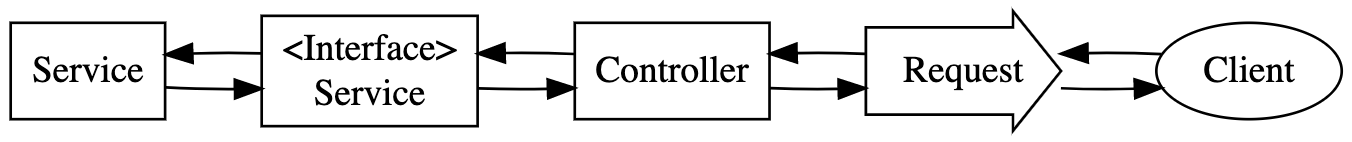
\includegraphics[width=\textwidth,height=\textheight,keepaspectratio]{images/patterns/service-controller}
\end{figure}

\subsubsection{API overview}
% TODO API diagrams and structure
\begin{figure}[H]
\caption{Forms controller endpoints}
\centering
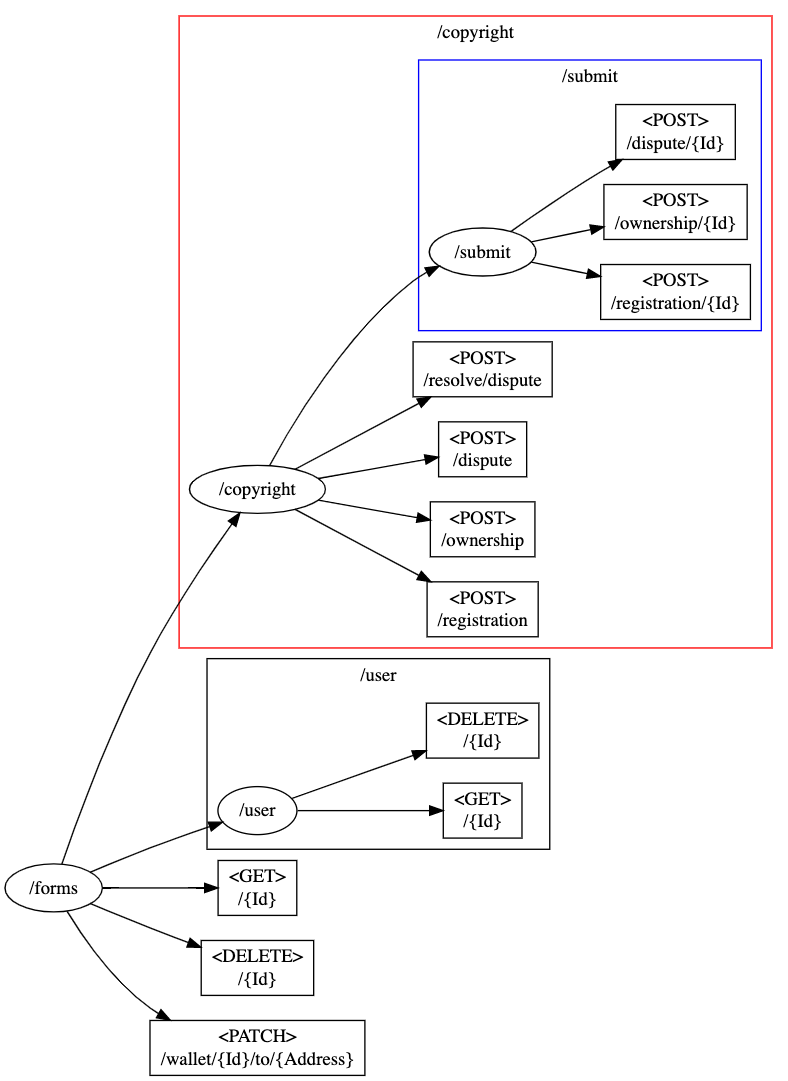
\includegraphics[width=\textwidth,height=0.5\textheight,keepaspectratio]{images/operational/Forms-Api}
\end{figure}

looking at the most complex and largest controller, I tried to keep the controller as \textit{RESTful} as possible with all endpoints describing the resource being accessed in conjunction with appropriate HTTP methods that describe the action performed on a resource.

\subsubsection{Applications framework}

The applications framework was built exploiting object oriented programming techniques mainly inheritance and polymorphism. An application has three classes each an implementation of each abstract base class, this means applications can be handled together generically and individually based on the child class.

\begin{figure}[H]
\caption{Application base class \href{https://github.com/MrHarrisonBarker/CRPL/blob/main/CRPL.Data/Applications/DataModels/Application.cs}{derived from}}
\centering
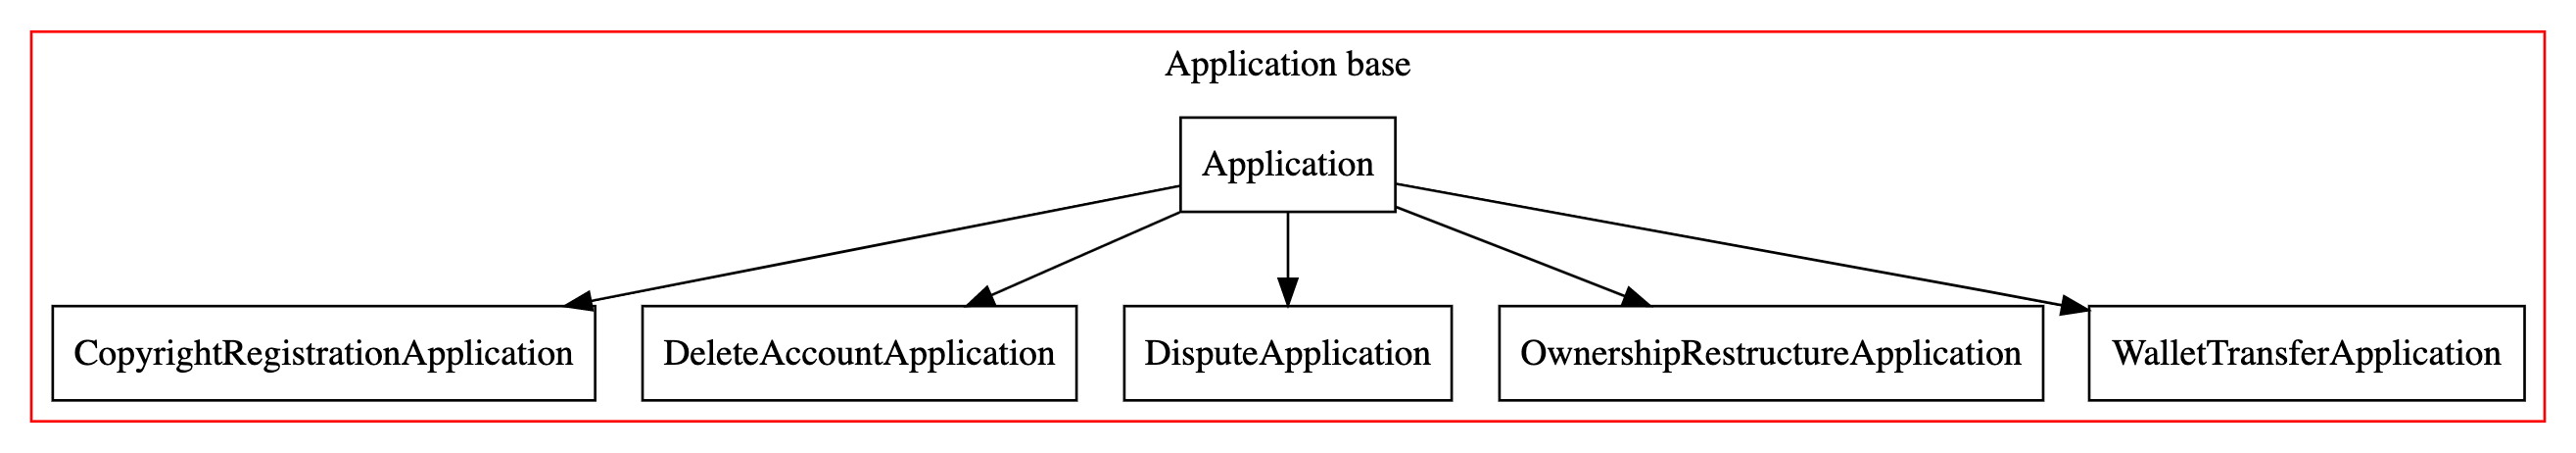
\includegraphics[width=\textwidth,height=0.5\textheight,keepaspectratio]{images/operational/application-base}
\end{figure}

This is the base \textit{Application} class and used by \textbf{EF Core} to generate database migrations creating and modifying tables. Therefore this class establishes all relationships, in this case a many to many with users and one to many with a registered work.

\begin{figure}[H]
\caption{Application view model class \href{https://github.com/MrHarrisonBarker/CRPL/blob/main/CRPL.Data/Applications/ViewModels/ApplicationViewModel.cs}{derived from}}
\centering
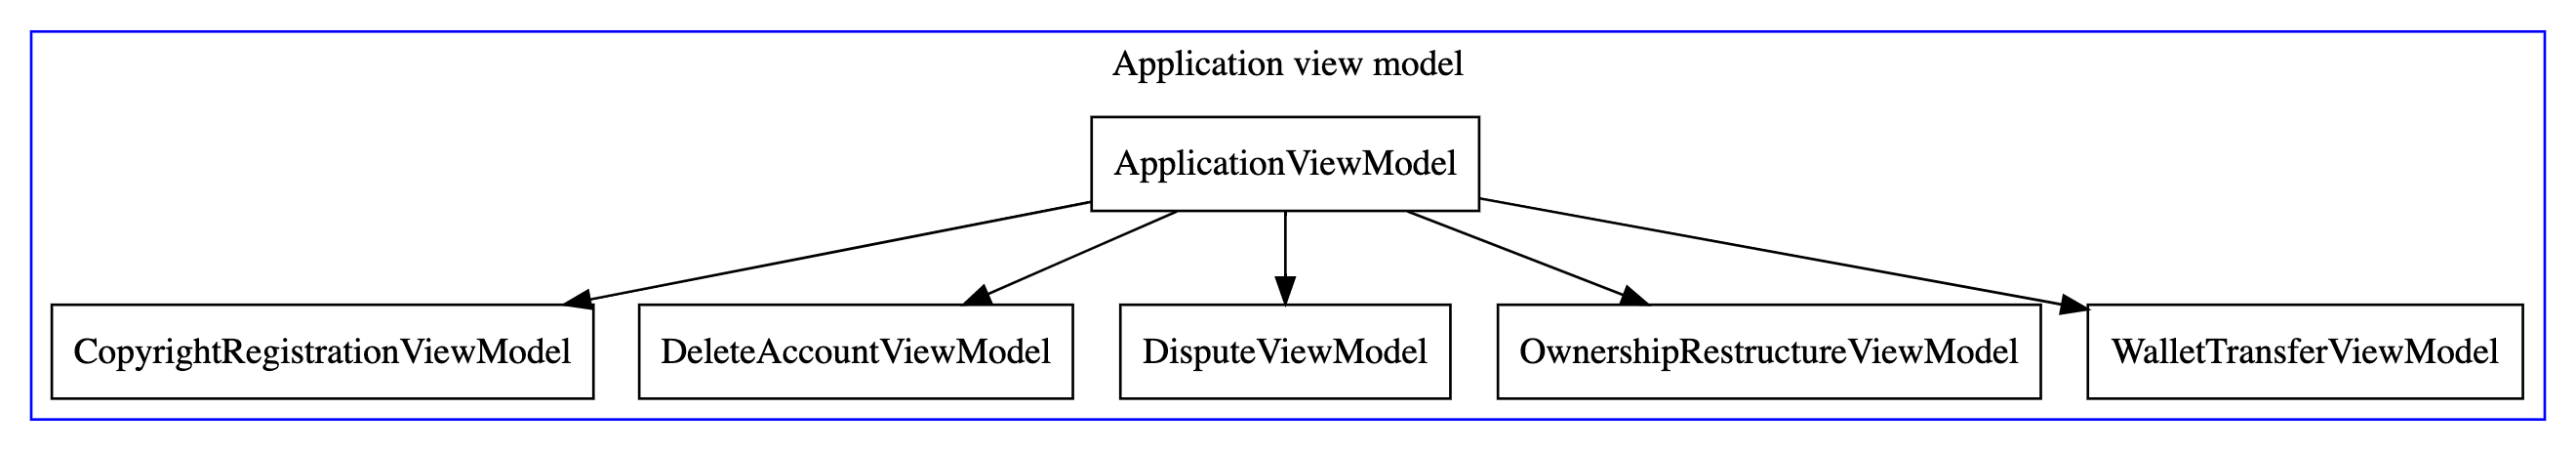
\includegraphics[width=\textwidth,height=0.5\textheight,keepaspectratio]{images/operational/application-view}
\end{figure}

The application view model is used when retrieving and displaying data, a lot of the time you don't want to send everything from the base model to the client or some processing/mapping maybe wanted. For applications the relationship between users is mapped from a junction table into a list of \textit{UserAccountMinimalViewModel}s
 
\begin{figure}[H]
\caption{Application input model class \href{https://github.com/MrHarrisonBarker/CRPL/blob/main/CRPL.Data/Applications/InputModels/ApplicationInputModel.cs}{derived from}}
\centering
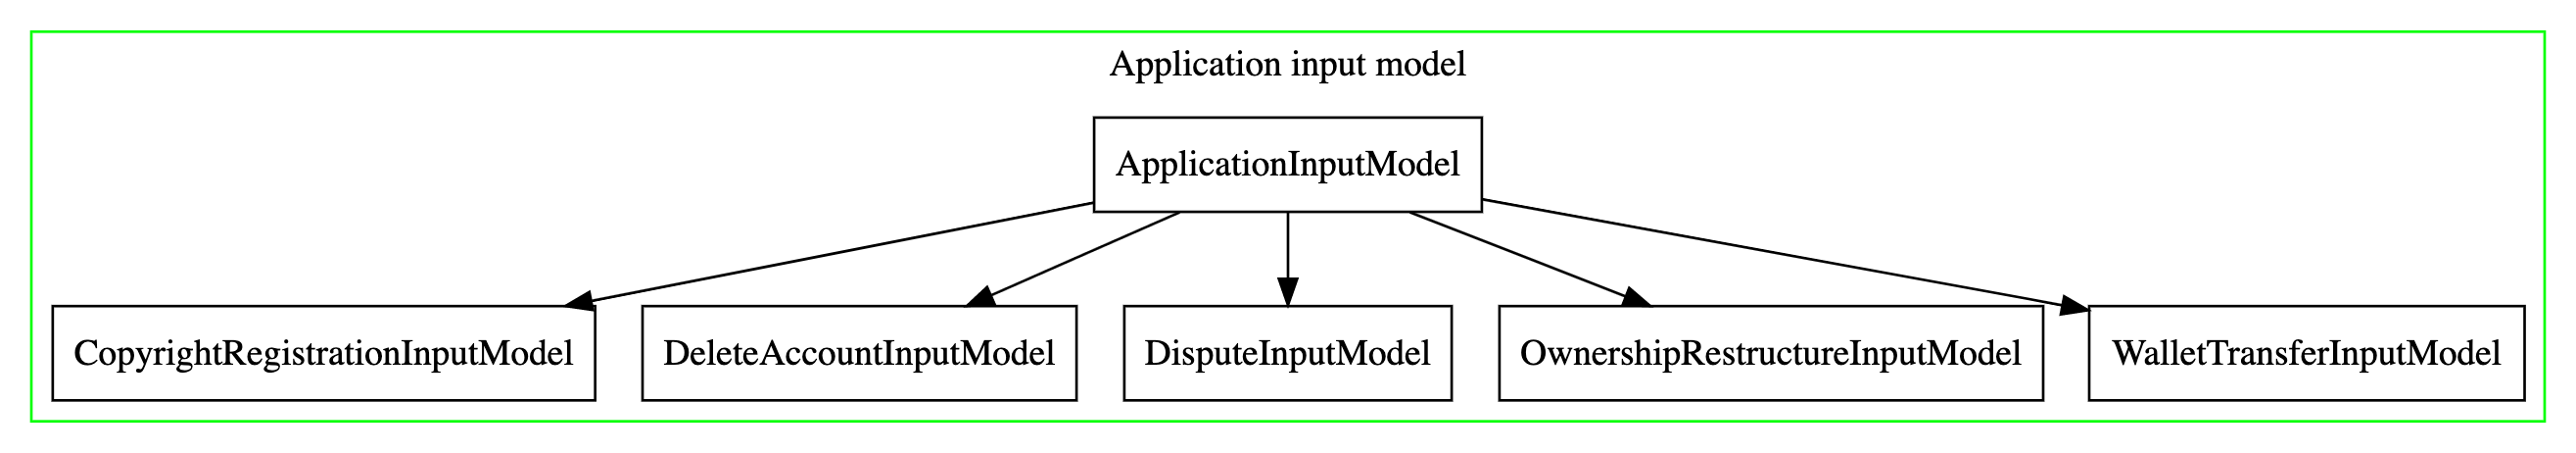
\includegraphics[width=\textwidth,height=0.5\textheight,keepaspectratio]{images/operational/application-input}
\end{figure}

Lastly an input model which is used when updating an application, this usually represents a real form the user is interacting with. This data is interpreted within the update method which modifies the data model on the database.
\br
One huge benefit of all applications using the same base class is that state can be generalised and kept consistent between different types of applications, a completed registration application should logically be the same as a completed dispute application.
This state can bee seen in the \textit{Applications framework} section of my design.

\begin{figure}[H]
\caption{Example application updater \href{https://github.com/MrHarrisonBarker/CRPL/blob/main/CRPL.Web/Core/Applications/Updaters/CopyrightRegistrationUpdater.cs}{CopyrightRegistrationUpdater}}
\centering
\begin{lstlisting}[language=CSharp]
public static class CopyrightRegistrationUpdater
{
    private static readonly List<string> Encodables = new() { "OwnershipStakes", "Id"  };
    
    public static async Task<CopyrightRegistrationApplication> Update(this CopyrightRegistrationApplication application, CopyrightRegistrationInputModel inputModel, IServiceProvider serviceProvider)
    {
        var userService = serviceProvider.GetRequiredService<IUserService>();
        
        application.UpdateProperties(inputModel, Encodables);

        if (inputModel.OwnershipStakes != null)
        {
            application.OwnershipStakes = inputModel.OwnershipStakes.Encode();

            application.CheckAndAssignStakes(userService, inputModel.OwnershipStakes);
        }

        return application;
    }
}
\end{lstlisting} 
\end{figure}

Each application also has an updater which is used for parsing the input model and updating the data model, this one is for the copyright registration application and is fairly simple. First it gets an instance of the user service, calls a static method I made that matches class properties between the input model and data model then updates those properties using the input model, complex object cant be saved in a db column so the ownership stakes are encoded into strings and then a relationship is updated/established between all the shareholders and the application.

\begin{figure}[H]
\caption{Example application submitter \href{https://github.com/MrHarrisonBarker/CRPL/blob/main/CRPL.Web/Core/Applications/Submitters/CopyrightRegistrationSubmitter.cs}{CopyrightRegistrationSubmitter}}
\centering
\begin{lstlisting}[language=CSharp]
public static class CopyrightRegistrationSubmitter
{
    public static async Task<CopyrightRegistrationApplication> Submit(this CopyrightRegistrationApplication copyrightRegistrationApplication, IServiceProvider serviceProvider)
    {
        var registrationService = serviceProvider.GetRequiredService<IRegistrationService>();
        
        await registrationService.StartRegistration(copyrightRegistrationApplication);

        copyrightRegistrationApplication.Status = ApplicationStatus.Submitted;
        
        return copyrightRegistrationApplication;
    }
}
\end{lstlisting}
\end{figure}

In addition to an updater applications need a submitter for when all the data has been inputted and is now ready to be processed, in the case of \textit{CopyrightRegistrationSubmitter} it starts the registration process (creates work and start verifying) and sets the status of the application to submitted. The majority of submitters start some background process or will require further processing to then be completed.

\subsubsection{Registration process}

The copyright registration process can be broken down into: fill and submit application, verification, send to chain and transaction verified.

\begin{figure}[H]
\caption{Registration state flow}
\centering
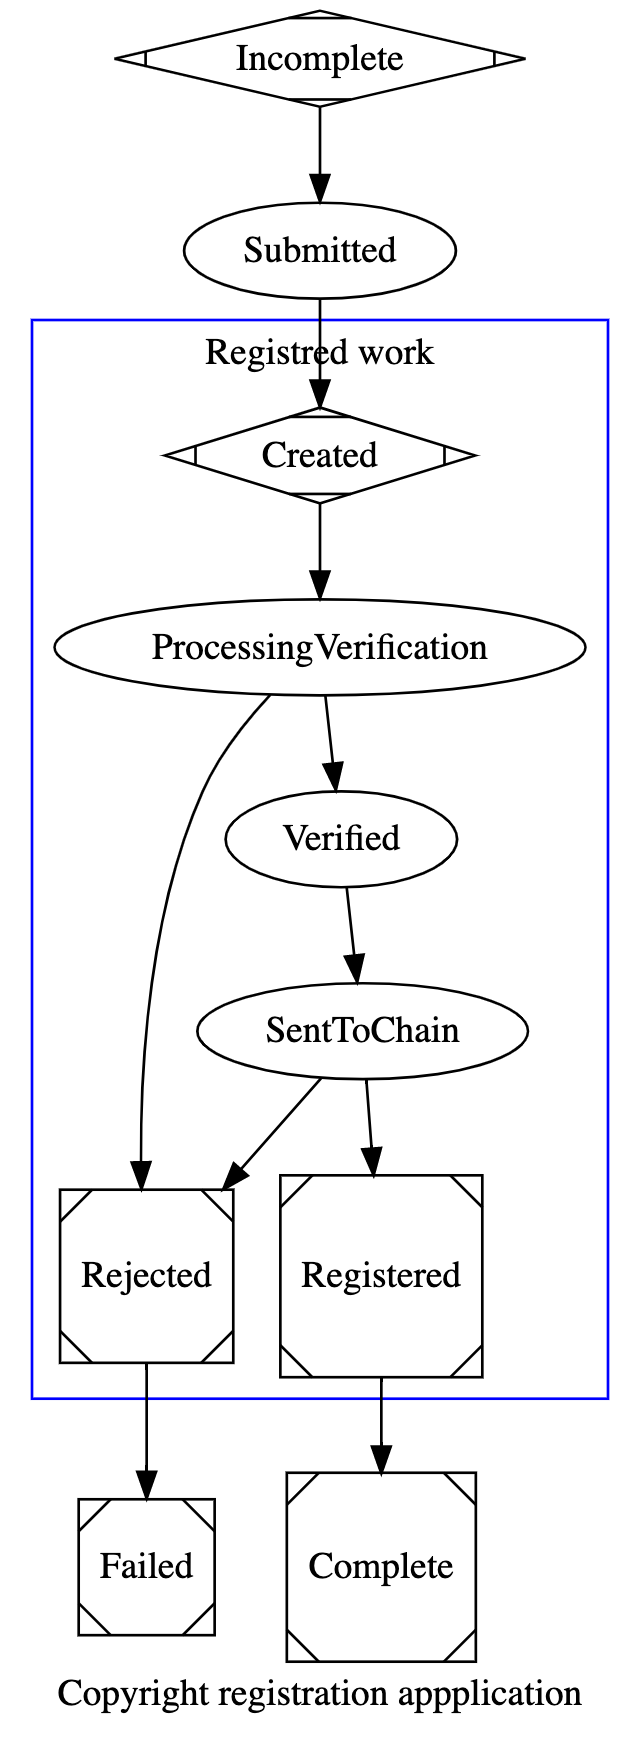
\includegraphics[width=\textwidth,height=0.5\textheight,keepaspectratio]{images/operational/cpy-registration-status-graph}
\end{figure}

The first step works as previously discussed, a user fills out a form/application submitting when all data has been inputted. validation of the data is handled on the client side with some server side sanity checks, this is reduce development workload and complexity however this is compromised by a user calling the API directly either maliciously or if I was to open up my API for public use.

% There is a section below talking about this step
\begin{figure}[H]
\caption{Finding collisions \href{https://github.com/MrHarrisonBarker/CRPL/blob/main/CRPL.Web/Services/WorksVerificationService.cs}{Line 57:58}}
\centering
\begin{lstlisting}[language=CSharp]
var collision = await Context.RegisteredWorks
           	.FirstOrDefaultAsync(x => x.Hash == work.Hash && x.Id != workId);
\end{lstlisting}
\end{figure}

Verification is handled by background service working though a queue which checks for collisions by comparing the uploaded work hash against all known work hashes. If a collision is found the application is set to \textit{Failed} and the work is set to \textit{Rejected}.

\begin{figure}[H]
\caption{Register message \href{https://github.com/MrHarrisonBarker/CRPL/blob/main/CRPL.Web/Services/RegistrationService.cs}{Line 88:102}}
\centering
\begin{lstlisting}[language=CSharp]
var register = new RegisterFunction()
{
	To = application.OwnershipStakes.Decode().Select(x => Mapper.Map<OwnershipStakeContract>(x)).ToList(),
	Meta = new Meta
	{
		Expires = new BigInteger((DateTime.Now.AddYears(application.YearsExpire) - new DateTime(1970, 1, 1, 0, 0, 0, DateTimeKind.Utc)).TotalSeconds),
		Title = application.Title,
		Registered = new BigInteger((DateTime.Now - new DateTime(1970, 1, 1, 0, 0, 0, DateTimeKind.Utc)).TotalSeconds),
		LegalMeta = application.Legal,
		WorkHash = Encoding.UTF8.GetString(application.WorkHash),
		WorkUri = application.WorkUri,
		WorkType = application.WorkType.ToString(),
		Protections = application.Protections
	}
};
\end{lstlisting}
\end{figure}

A \keyword{copyright} is then sent to the \keyword{blockchain} when a shareholder sends a complete request, this creates a register message (seen above) and sends it to the chain returning a transaction hash which is stored for later reference.

\begin{figure}[H]
\caption{Registered Event Processor \href{https://github.com/MrHarrisonBarker/CRPL/blob/main/CRPL.Web/Core/EventProcessors/RegisteredEventProcessor.cs}{Line 29:31}}
\centering
\begin{lstlisting}[language=CSharp]
context.Update(registeredWork);

registeredWork.RightId = registeredEvent.Event.RightId.ToString();
registeredWork.Registered = DateTime.Now;
registeredWork.Status = RegisteredWorkStatus.Registered;

registeredWork.AssociatedApplication.First(x => x.ApplicationType == ApplicationType.CopyrightRegistration).Status = ApplicationStatus.Complete;	
\end{lstlisting}
\end{figure}

Verifier and miner nodes on the network will now process this transactions, this takes an indeterminate time based on how much money you want to spend and the current capacity of the network. Once verified and processed into the chain a \textit{Registered} event will be picked up by the event processors running, the processor will match the transaction hashes setting the work to registered and its registration application to complete.

\subsubsection{Queries - Chain injection}
% TODO structured query

\begin{figure}[H]
\caption{Data injection from \keyword{blockchain} when querying registered works}
\centering
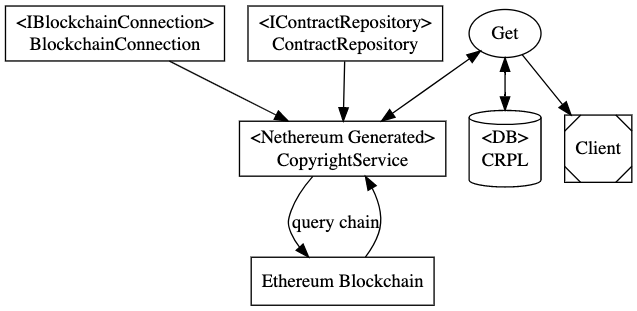
\includegraphics[width=\textwidth,height=\textheight,keepaspectratio]{images/operational/chain-inject}
\end{figure}

Because I rely on the \keyword{blockchain} as the store and point of truth in the system I need a way of querying a \keyword{copyright} for data to display to the user. 

\begin{figure}[H]
\caption{Metadata query from query service \href{https://github.com/MrHarrisonBarker/CRPL/blob/main/CRPL.Web/Services/QueryService.cs}{Line 155:156}}
\centering
\begin{lstlisting}[language=CSharp]
var meta = await new Contracts.Copyright.CopyrightService(BlockchainConnection.Web3(), ContractRepository.DeployedContract(CopyrightContract.Copyright).Address)
		.CopyrightMetaQueryAsync(rightId);
...
registeredWork.Meta = meta != null ? meta.ReturnValue1 : null;
\end{lstlisting}
\end{figure}

This is apart of a big function called \textit{injectFromChain} found in the \href{https://github.com/MrHarrisonBarker/CRPL/blob/main/CRPL.Web/Services/QueryService.cs}{query service} and is called whenever a work is requested from the service, it queries the \keyword{blockchain} for data then "injects" the found data into the existing registered work data model.

\subsubsection{Dispute handling}
% TODO filing disputes
% TODO resolving disputes: payment, change of ownership
\begin{figure}[H]
\caption{CAPTION}
\centering
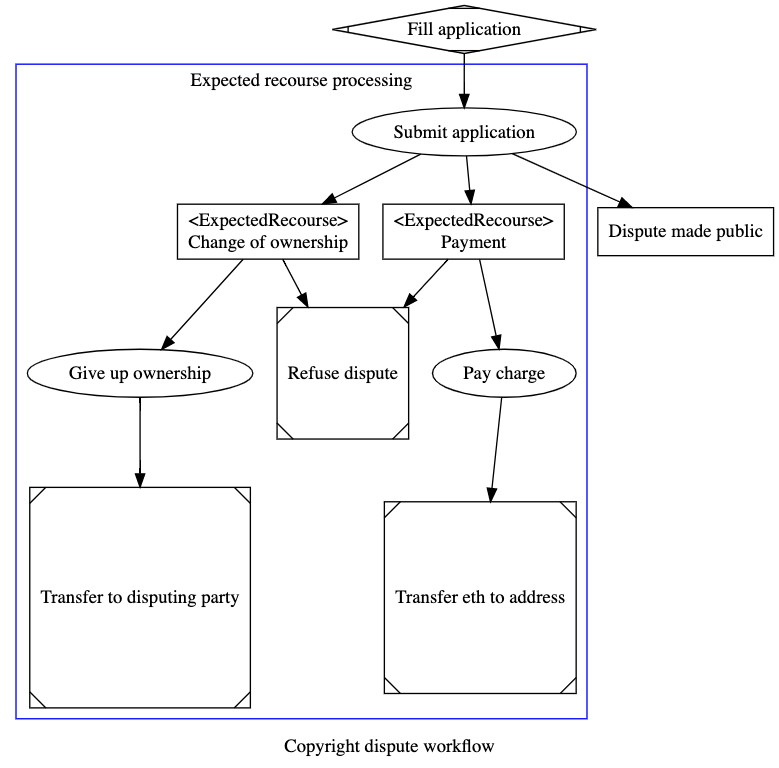
\includegraphics[width=\textwidth,height=\textheight,keepaspectratio]{images/operational/dispute-workflow}
\end{figure}

\subsubsection{Blockchain event listeners}
% TODO Blockchain event listeners

To listen for events in the \keyword{blockchain} \textbf{Nethereum} has a class called \textit{BlockchainProcessor} which listens for an event and registers a callback/action that is run when that specific event is found.

\begin{figure}[H]
\caption{Registering an event listener for \textit{Registered} event \href{https://github.com/MrHarrisonBarker/CRPL/blob/main/CRPL.Web/Services/Background/BlockchainEventListener.cs}{Line 32:33}}
\centering
\begin{lstlisting}[language=CSharp]
BlockchainConnection.Web3().Processing.Logs
	.CreateProcessorForContract<RegisteredEventDTO>(ContractRepository.DeployedContract(CopyrightContract.Copyright).Address, log => EventQueue.QueueEvent(log))
\end{lstlisting}
\end{figure}

For my system I'm using event processors that listen to a specific event type from a specific \keyword{smart contract}, see above this processor is listening for events of type \textit{RegisteredEventDTO} from the deployed contract retrieved from the \textit{ContractRepository}.

All my processors push all events to the event queue to be processed by a service instead of processing in the callback, this increases scaleability and breaks the code down into smaller modular chunks.

Events are pulled from the queue by the \href{https://github.com/MrHarrisonBarker/CRPL/blob/main/CRPL.Web/Services/Background/EventProcessingService.cs}{EventProcessingService} then processed by a \href{https://github.com/MrHarrisonBarker/CRPL/tree/main/CRPL.Web/Core/EventProcessors}{EventProcessor} which are static classes with one method \textit{ProcessEvent}, one is built for every event type listened to. 

\begin{figure}[H]
\caption{Processing events based on type \href{https://github.com/MrHarrisonBarker/CRPL/blob/main/CRPL.Web/Services/Background/EventProcessingService.cs}{Line 32:49}}
\centering
\begin{lstlisting}[language=CSharp]
switch (nextEvent.GetType().FullName)
{
	case var name when name.Contains("RegisteredEvent"):
		await ((EventLog<RegisteredEventDTO>)nextEvent).ProcessEvent(ServiceProvider, Logger);
		break;
	case var name when name.Contains("ApprovedEvent"):
		await ((EventLog<ApprovedEventDTO>)nextEvent).ProcessEvent(ServiceProvider, Logger);
		break;
	case var name when name.Contains("ProposedRestructureEvent"):
		await ((EventLog<ProposedRestructureEventDTO>)nextEvent).ProcessEvent(ServiceProvider, Logger);
		break;
	case var name when name.Contains("RestructuredEvent"):
		await ((EventLog<RestructuredEventDTO>)nextEvent).ProcessEvent(ServiceProvider, Logger);
		break;
	case var name when name.Contains("FailedProposalEvent"):
		await ((EventLog<FailedProposalEventDTO>)nextEvent).ProcessEvent(ServiceProvider, Logger);
		break;
}
\end{lstlisting}
\end{figure}

\subsubsection{Verification pipeline}
% TODO verification pipeline

The verification pipeline uses by background service architecture with a \textit{VerificationQueue} and \textit{VerificationPipelineService} that dequeues and processes verification of a work. 

\begin{figure}[H]
\caption{Verification pipeline}
\centering
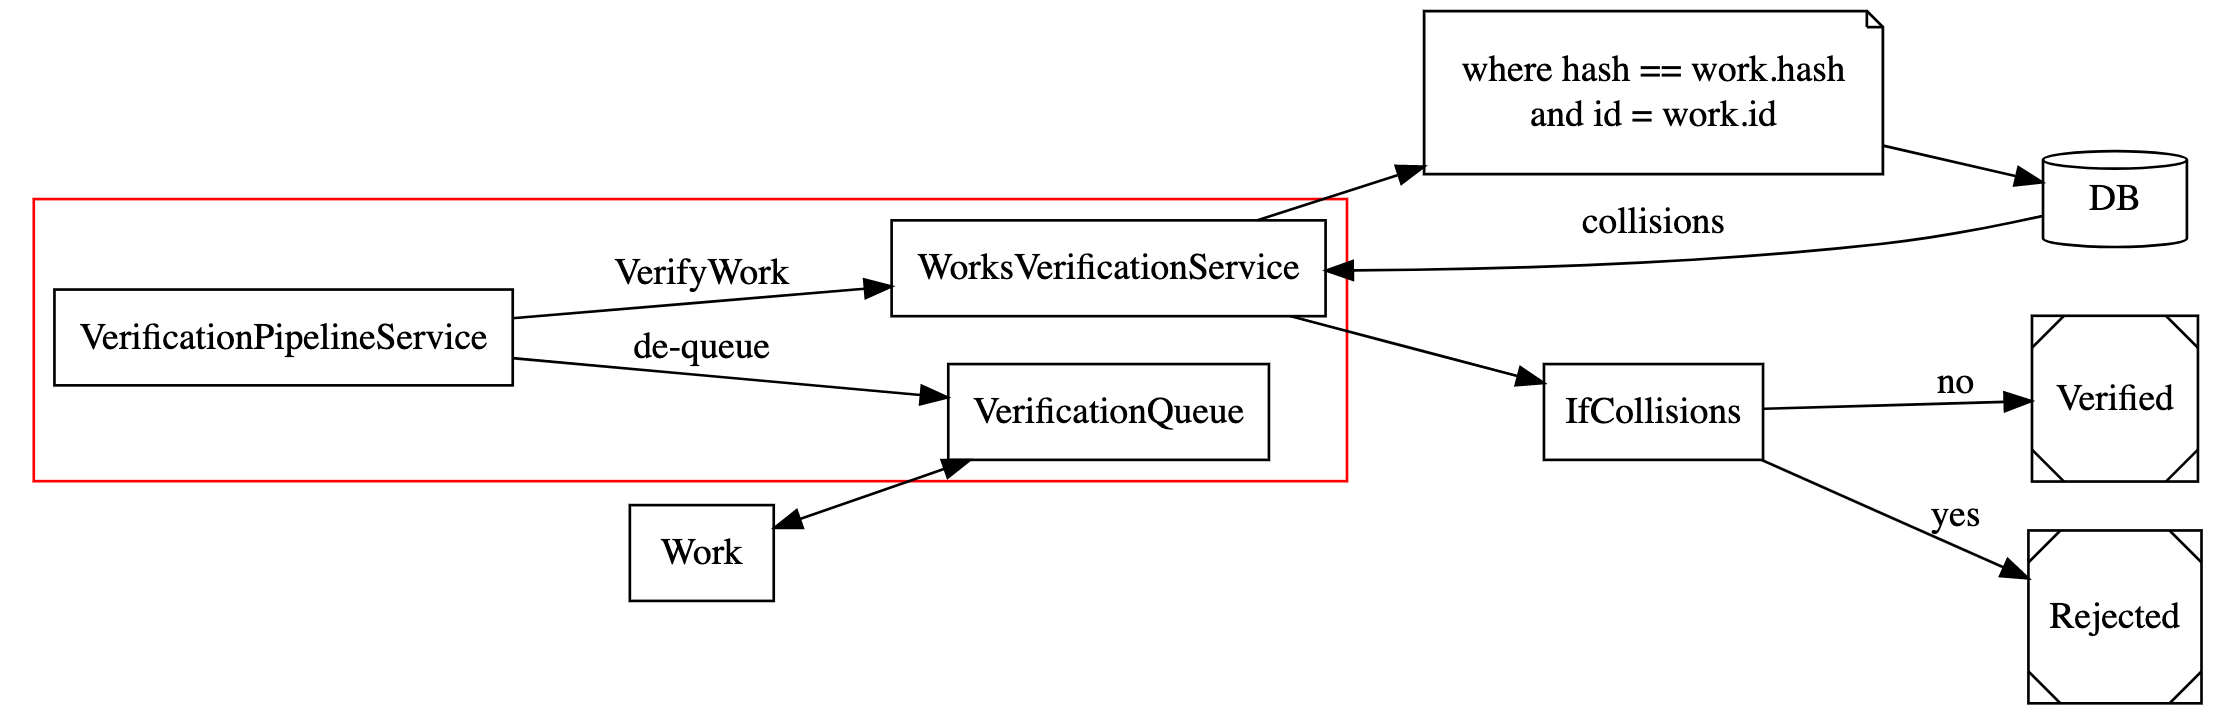
\includegraphics[width=\textwidth,height=\textheight,keepaspectratio]{images/operational/verification-pipe}
\end{figure}

% bit bad
When a work is pulled off the queue it is verified using the \href{https://github.com/MrHarrisonBarker/CRPL/blob/main/CRPL.Web/Services/WorksVerificationService.cs}{WorksVerificationService} method \textit{VerifyWork} which searches the database for existing works with the same hash. If no collisions are found the works status is updated to \textit{Verified}, if collision are found then the work is set to \textit{Rejected}

\begin{figure}[H]
\caption{hashing a work \href{https://github.com/MrHarrisonBarker/CRPL/blob/main/CRPL.Web/Services/WorksVerificationService.cs}{Line 146:151}}
\centering
\begin{lstlisting}[language=CSharp]
private byte[] HashWork(byte[] work)
{
	using var hashAlgorithm = SHA512.Create();

	return hashAlgorithm.ComputeHash(work);
}
\end{lstlisting}
\end{figure}

For hashing the uploaded work I stream the file into a byte array and compute the hash using \textbf{SHA-512} which has \(2^{512}\) total possible hash outputs which is \(1.34 \times 10^{154}\) almost double the number of atoms in the universe at around \(10^{82}\) so the possibility of a collision or exploitation is extremely low. 

Although \textbf{MD5} is mostly commonly used for very quick file duplicity checks these checks are usually just checksums to check file integrity of downloaded files. In terms of cryptographic security \textbf{SHA-512} is far better, \textbf{MD5} has been "broken" for years so should never be used for any sensitive or secure data hashing this is while the latest \textbf{SHA} algorithms are considered secure and are used in conjunction with "salt" for passwords in many systems.

\subsubsection{Account management}
% TODO issues with transfer and delete account

% TODO Expiry

\subsection{Database}

I've chosen to use a \textbf{MySQL} database for this project for two reasons: ease of use and \textbf{ACID}. Having previously used \textbf{MySQL} for multiple projects in the past plus the brilliant integration between \textbf{EFCore}, \textbf{LINQ} and \textbf{SQL}. \textbf{ACID} standing for \textbf{a}tomicity, \textbf{c}onsistency, \textbf{i}solation and \textbf{d}urability which ensure data integrity at the cost of speed over a \textit{NoSql} approach like \textbf{MongoDB}, it also has support for rigid relationships between entities.

\br

As talked about previously some data in the database has to be kept in parity with the \keyword{Blockchain} by querying the the deployed contract.

\begin{figure}[H]
\caption{ChainSync}
\centering
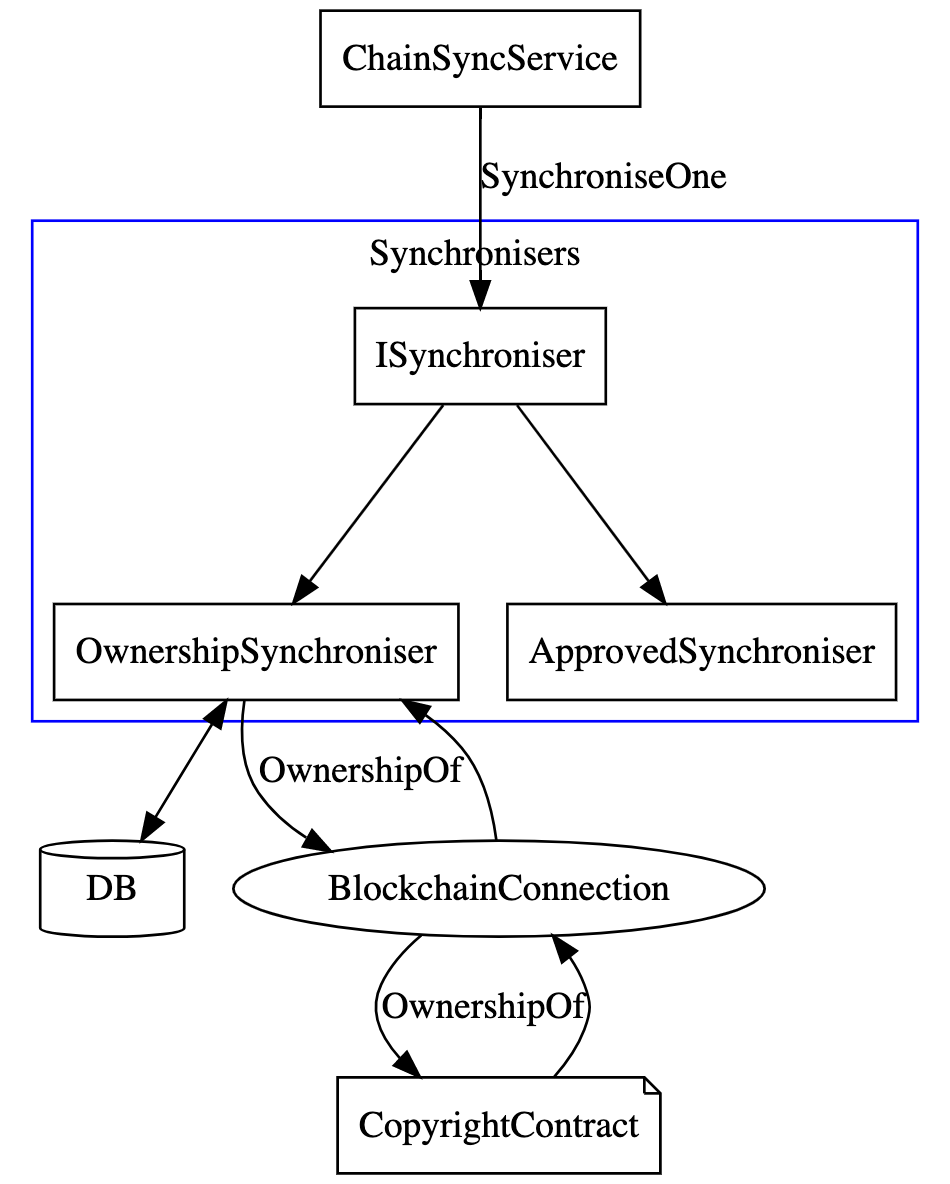
\includegraphics[width=\textwidth,height=0.5\textheight,keepaspectratio]{images/operational/chain-sync}
\end{figure}

Therefore a background service was built that synchronises all the \keyword{copyrights} currently being tracked with the \keyword{blockchain}, the service checks for changes on startup and then every 24 hours after startup.

\begin{figure}[H]
\caption{24 hour sync timer \href{https://github.com/MrHarrisonBarker/CRPL/blob/main/CRPL.Web/Core/ChainSync/ChainSyncService.cs}{Line 25:30}}
\centering
\begin{lstlisting}[language=CSharp]
CronTimer = new Timer(
	Sync,
	null,
	TimeSpan.Zero,
	TimeSpan.FromHours(24)
);
\end{lstlisting}
\end{figure}

There's only one synchroniser implemented in the system for ownership structures, it queries the \keyword{blockchain} using \textit{OwnershipOf} which is a method on the contract that returns an ownership structure for a specific \keyword{copyright}. It then checks against what is saved in the database, if changes are found relationships need to be removed and updated.

\begin{figure}[H]
\caption{ownership similarity \href{https://github.com/MrHarrisonBarker/CRPL/blob/main/CRPL.Web/Core/ChainSync/Synchronisers/OwnershipSynchroniser.cs}{Line 71, 77:86}}
\centering
\begin{lstlisting}[language=CSharp]
if (ownerships.Count != work.UserWorks.Count || !work.UserWorks.All(x => ownerships.Contains(x.UserAccount.Wallet.PublicAddress.ToLower())))
...
work.UserWorks.Clear();
ownerships.ForEach(async owner =>
{
	var user = await Context.UserAccounts.FirstOrDefaultAsync(x => x.Wallet.PublicAddress.ToLower() == owner.ToLower());
	if (user == null) throw new UserNotFoundException(owner);
	work.UserWorks.Add(new UserWork()
	{
		UserAccount = user
	});
});
\end{lstlisting}
\end{figure}

\subsection{Front-end}

A fancy UI was not a high priority of this project as the core back-end and \keyword{blockchain} interaction is expansive and complex enough in isolation, however I wanted to at least give a user the ability to interact with the system I've built hopefully in a usable and accessible way.

Most user interface design thought and work was spent on the four key forms (user register, copyright register, ownership restructure and dispute) as from previous experience forms are the hardest piece (for me) of interface design by far. To make this easier I counter intuitively at first did not care about the design or usability of the components I was building only getting the data into the form and sent off to the back-end.

This produced some initial designs that functionally work but were confusing for a new user and just didn't look very nice, I've found it's very easy to get hung up on user interface when building systems\footnote{I think this is down to the fact that it's the single point of contact with your users, most people will not see and or care about business logic code but how your interface looks and feels are front and centre. this would be okay in a real product development setting but for this project it's just not within the scope.} which slows down development especially in the early stages of development when the constraints and needs of the system are changing.

Then after all core features had been built I then went back to my forms and re-designed all input components using a consistent set of rules, requirements and style.    

\begin{figure}[H]
\caption{Example input markup \href{https://github.com/MrHarrisonBarker/CRPL/blob/main/CRPL.Web/ClientApp/src/app/Forms/cpy-registration-form/cpy-registration-form.component.html}{cpy-registration-form.component.html 9:18}}
\centering
\begin{lstlisting}[language=html]
<div class="input-container">
	<label class="input-label">Title<sup>*</sup></label>
	<div class="input-control">
	<input type="text" name="title" formControlName="Title" placeholder="Hello world"/>
	<div>This is a searchable title for the copyright, it doesn't have to be unique only descriptive and relevant&nbsp;<sup>*saved to the blockchain</sup></div>
		<clr-alert class="input-error" [clrAlertClosable]="false" clrAlertType="danger" *ngIf="InvalidAndUntouched('Title')">
		 	<clr-alert-item>This field is required!</clr-alert-item>
	 </clr-alert>
	</div>
</div>
\end{lstlisting}
\end{figure}

Below is the my \href{https://github.com/MrHarrisonBarker/CRPL/tree/main/CRPL.Web/ClientApp/src/app/Forms/ownership-structure-form}{ownership-structure-form} component that's used in both \href{https://github.com/MrHarrisonBarker/CRPL/tree/main/CRPL.Web/ClientApp/src/app/Forms/cpy-registration-form}{cpy-registration-form} and \href{https://github.com/MrHarrisonBarker/CRPL/tree/main/CRPL.Web/ClientApp/src/app/Forms/cpy-restructure-form}{cpy-restructure-form}, this means all forms have to be consistent across the application so any section of a form will "fit" into any other form.

\begin{figure}[H]
\caption{\href{https://github.com/MrHarrisonBarker/CRPL/tree/main/CRPL.Web/ClientApp/src/app/Forms/ownership-structure-form}{Ownership structure form} component}
\centering
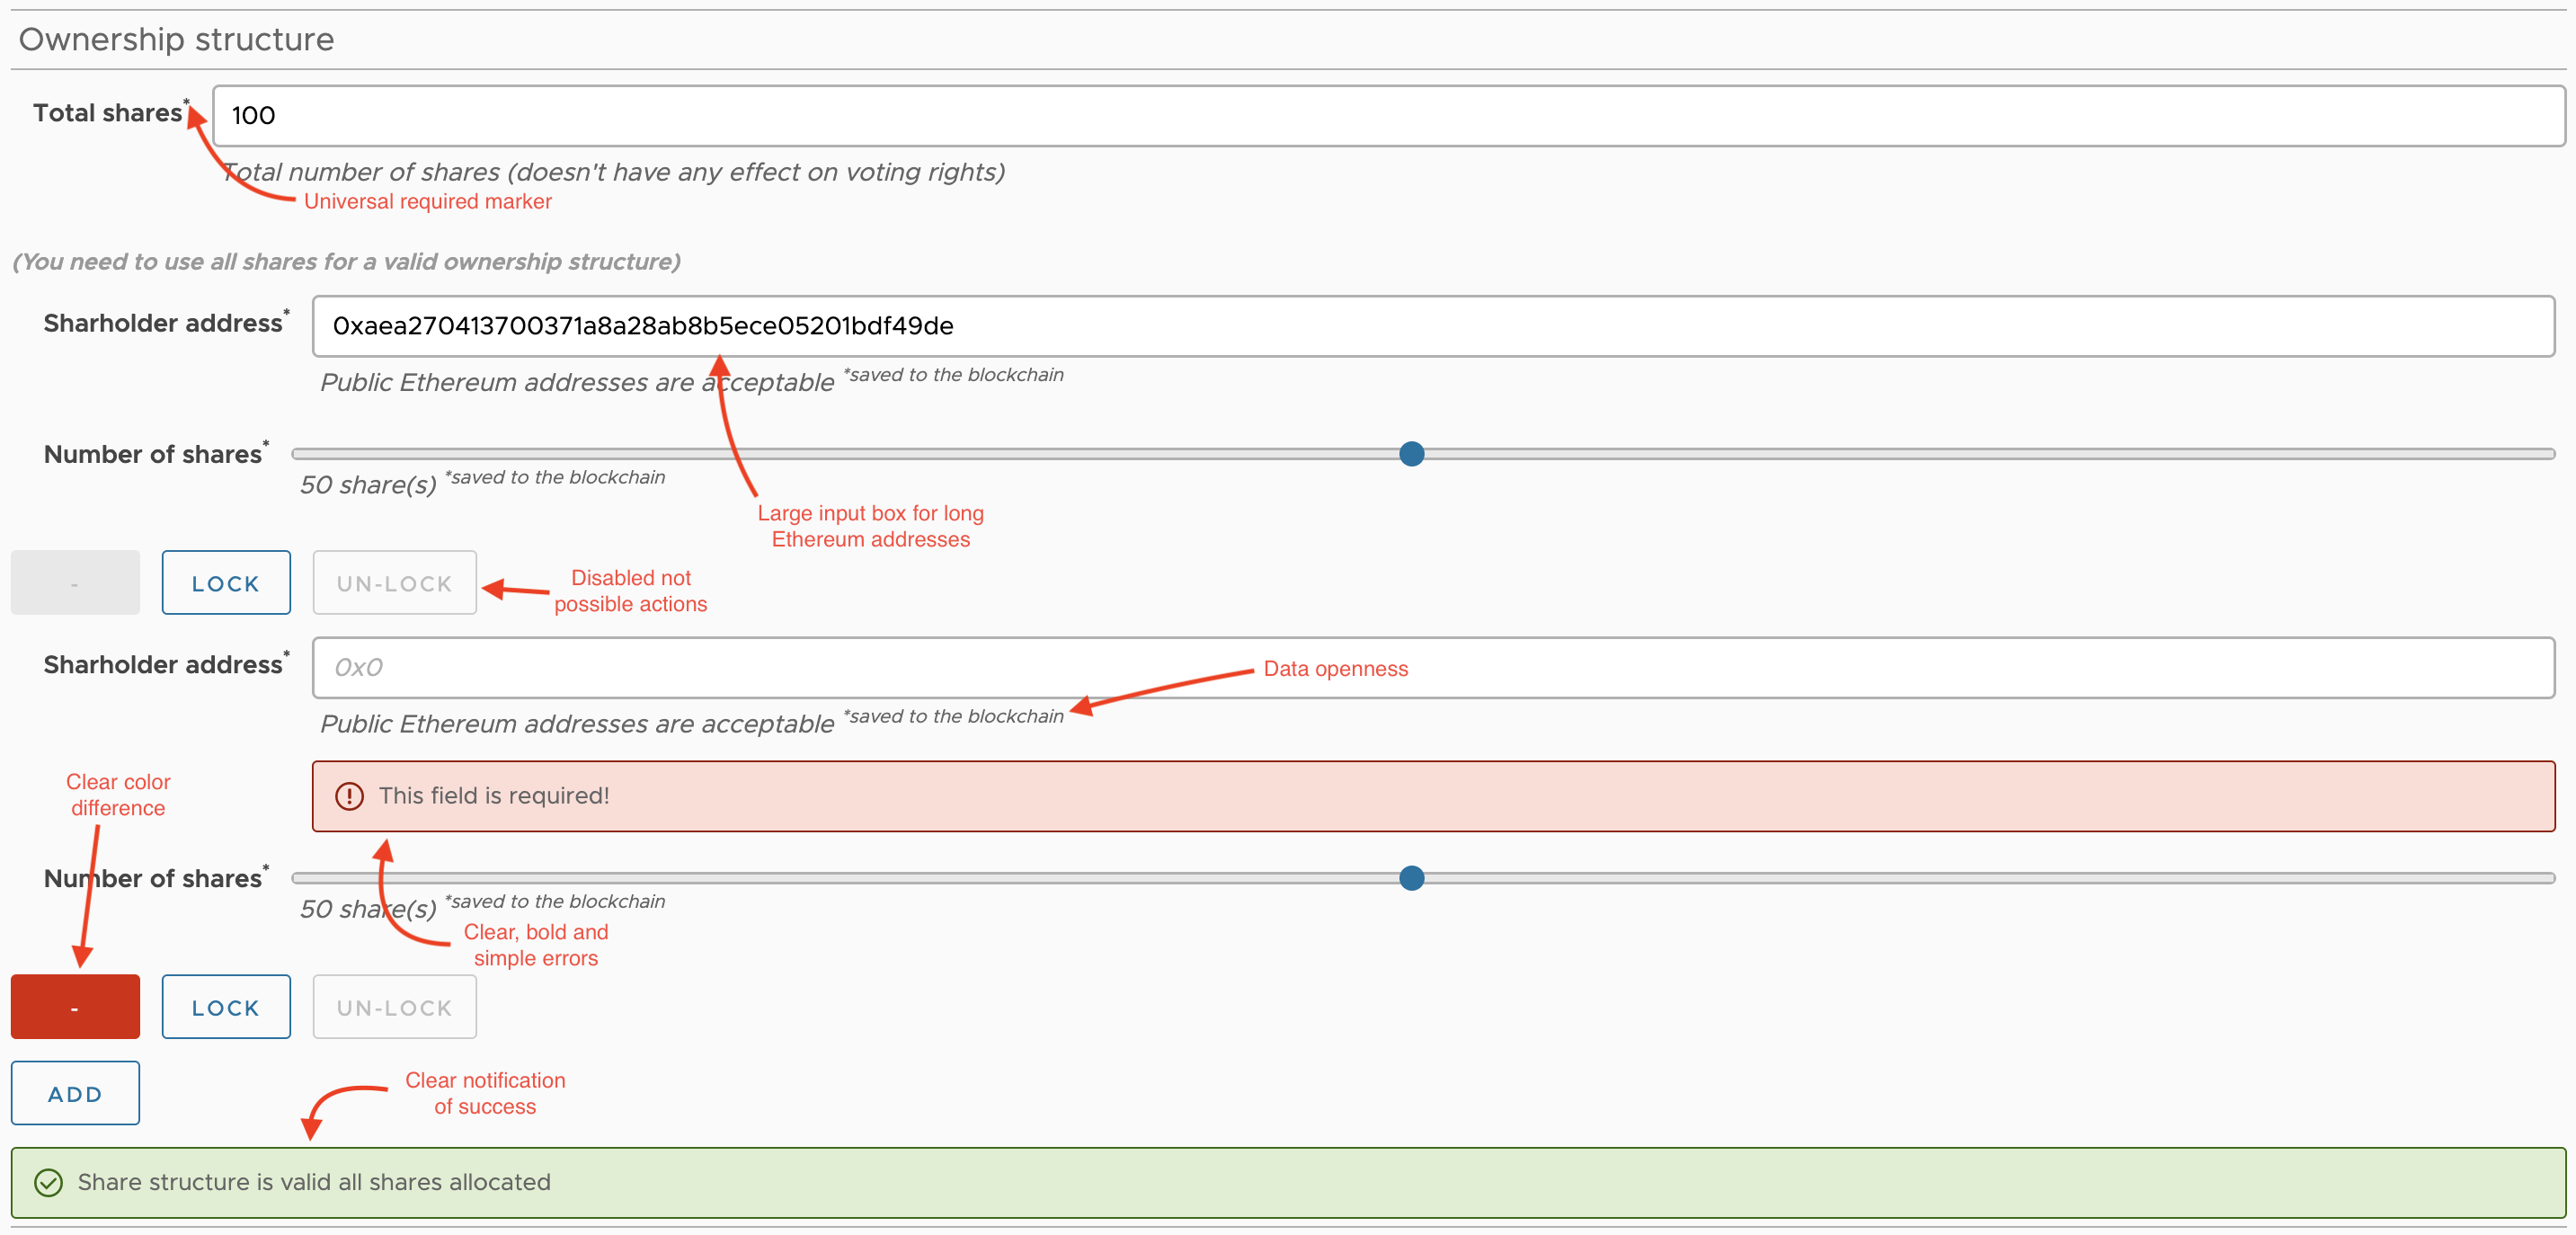
\includegraphics[width=\textwidth,height=\textheight,keepaspectratio]{images/wireframe/ownership-structure}
\end{figure}

\section{Discussion}
\subsection{Limitation}
% TODO limits of the scope (having to reign in the scope of the project at all points)
% TODO limits of the implementation (gas/price aka no money involved at the moment, transfer and delete wallet, de-sync)
% TODO no way of licences for the use of a work

\subsection{Blockchain technology}
% TODO Are these NFTs?
% TODO How long will the blockchain?
% TODO Social consensus/ conflict with governments

\section{Evaluation}
\subsection{Process}
% TODO evaluating my development
% TODO was development agile?

\subsection{Product}
% TODO Has all the functional specifications been met
% TODO Has all the non-functional specs been met
% TODO Does the product fit the target users needs
% TODO Does the product fulfil

% TODO TESTING TESTING TESTING

\section{Future development}

\begin{description}
	\item[Royalty payments]
	\item[External verification]
	\item[Analytics]
\end{description}

\section{Conclusion}


\bibliographystyle{plain}
\bibliography{sources.bib}

\end{document}
